%
% Copyright (c) 2008  Betti Österholz
%
% Permission is granted to copy, distribute and/or modify this document
% under the terms of the GNU Free Documentation License, Version 1.2 or
% any later version published by the Free Software Foundation;
% with no Invariant Sections, no Front-Cover Texts, and no Back-Cover Texts.
%
% A copy of the license is included in the file ``fdl.tex'' .
%

%path for pictures
\graphicspath{{./stock_language_description/}}
\graphicspath{{./stock_language_description/}{../stock_language_description}}


\newpage
\part{The Fib multimedia description language}
\label{partFibLanguage}

In this part the elements of the Fib multimedia language will be defined.


\section{Requirements}
\label{secFibLanguageRequirements}

Since for the classical bit representation low performance can be expected by genetic algorithms, but because of the complexity of the problem a very high performance is needed, an adapted problem representation (multimedia description language) is selected.

The multimedia description language Fib should be kept as simple as possible, with yust few alternatives, since an increases of the available alternatives will increase the number of alternatives in the application of the genetic operations and this will likely increase the amount of computation and implementation complexity.

On the other side, the multimedia description language should allow compact expressions for ``normal'' (occurring in the practice) multimedia objects. It should therefore provide good compression options for `` normal'' multimedia objects. This implies that relationships (e. g. color gradients in a surface) between parts (e. g. pixels of the surface) of a multimedia object can be represented as simply as possible.

The language should be unambiguous, reproducible and evaluable, so that an expression always evaluates to the same object. The clarity and reproducibility isn't so important for the implementation (e. g. due to different rounding errors on different architectures), if the generated multimedia object is almost always (as an example, in $0.999999$ fraction of cases) very similar to the original multimedia object. But valid language objects have to be always evaluable. Otherwise restrictions on the genetic operators, by which they wher generated, have to be made or not evaluable objects could arise.

With the multimedia description language it should be possible to represent at least all raster graphics.
The generation of a raster image by a Fib multimedia object in the multimedia description language should be comprehensible. That is, the multimedia description language should be designed to support the distinction of individual objects and their dependencies.

The genetic operations which change the multimedia programs should, if possible, change the program in a way, to allow a gradient descent in the hypothesis space of the multimedia programs. By running multiple operators the hypotheses, that the multimedia programs represent, should therefore be gradually improved.


\section{The multimedia description language}

The multimedia description language is named Fib (for ``funktionale Interpretation von Bildern'' or ``functional interpretation of bitmaps (/bictures)''). This name orgins from the first version of the multimedia description language, when it was only good for saving images (german: Bilder).

With some additional elements the multimedia description language has been extended, so that it can store any multimedia data. The only restriction on the multimedia data is, that it can be represented as properties of points of a finite, euclidean and discrete (there are smallest units) space.

Fib is a vector representation of multimedia data, that means a representation of multimedia data using objects.
As a basic framework a tree is used. The leaves are endpoints that are used for displaying and / or assignment of points or part of multimedia objects. In the branches and the alignment of these, which for example is most left, display parameters or properties of the leaves are encoded, e. g. how often it is displayed or with which color.

Each node of the tree is a Fib element. The tree is evaluated from the root to the leaves, whereupon the elements affect the evaluation.

A valid Fib object (tree) is cycle free, to ensure a finite processing time.

The elements of the multimedia description language are oriented on some of the usual imperative programming languages (e. g. C++, Java).

All units are expressed on the basis of the International System of Units (SI).

When a Fib object is evaluated, all points with their properties are determined for the multemedia object. A evaluated multimedia object thus contains only a list of specific points and their properties, and can thus be directly displayed (through displaying the properties at the points / coordinate) or evaluated.

Hereinafter ``top'' in the Fib object is referred to the direction, in which the root of the tree lies. The direction of ``bottom'' is thus the opposite direction (away from the root).


\section{Elements of the Fib multimedia description language}
\label{secFibElements}

This section describes the elements of the Fib multimedia description language.

Below $Obj$ stands for a Fib object.


\subsection{Vectors}

Vectors are used for providing numerical values. There are different types of vectors (e. g. position vectors, range vectors or property vectors for RGB colors). The type of a vector (and optionally information in the root-element) gives the domain and the number of the elements that it contains.
Each vector element is either a number or a variable, which is set in the Fib object above the Fib element of the vector.

If the value of an evalued element is outside of its domain (the domain for the vector element), this value is rounded to the nearest value that lies in the domain.
If an element of the vector is not existing, it is evaluated as the zero value of its domain.

Vectors of one type are only used in a very specific type of Fib element.

A listing of the possible vector typs can be found in Table \ref{tableVectorTyps} .


\begin{table}[htbp]
\begin{center}
\begin{tabular}{|p{20mm}|p{35mm}|p{15mm}|p{20mm}|p{15mm}|}\hline
	vector & description & used in Fib element & number of elements & typ of elements \\\hline\hline
	position & the position of a point & $point$ & any (a vectors can always contain just 0 elements) & numbers \\\hline
	area & contains the borders of an area (inclusive the borders) & $area$ & 2 & integers \\\hline
	property vector (there are more than one type) & defines a value of a property & $property$ & any & numbers \\\hline
\end{tabular} 
\end{center}
\caption{Vector typs}
\label{tableVectorTyps}
\end{table}


\subsection{Points}\index{point element|(}
\label{fibPoint}\label{secFibPoint}

The points are the displaying elements. At them the set properties are evaluated. Points serve as the leaves of Fib objects.

An empty point ``point()'' is possible. The empty point has no effect (all properties are lost). It can be used in combination with other elements (e. g. the if-element).

There are also points with an empty position vectors ``point(())'', these points create the background (e. g. the background color).

The properties of the point (e. g. color, sound and / or odor) are determined in the branch above the point with property elements.

\bigskip\noindent
Syntax:
$Obj = point( PositionVector )$

\bigskip\noindent
Short syntax:
$Obj = p( PositionVector )$

\begin{description}
 \item[$PositionVector$]: the coordinate vector of the point
\end{description}

\bigskip\noindent
Examples:
\begin{itemize}
 \item $p((10;20))$; a point on the position $(10,20)$
 \item $p((10;x))$; $x$ is a variable that must be set in the branch to this point
 \item $p()$; the point has no impact and all the properties are discarded
 \item $p(())$; point that affects the entire background
\end{itemize}

\index{point element|)}


\subsection{Property element}\index{propertie element|(}
\label{fibProperty}\label{secFibProperty}

With the property element ``property'' properties for Fib objects will be set.

\bigskip\noindent
Syntax:
$Obj = property( ( value_1, ..., value_n)_{name}, Obj_1 ) $

\bigskip\noindent
Short syntax:
$Obj = pr( (value_1, ..., value_n)_{name}, Obj_1 )$

\begin{description}
 \item[$name$] The $name$ specifies the name of the property. It determines the type of the vector. All property types should belong to the vector supertype ``property''.
 \item[$value_i$] This is the value $i$ of the property.
 \item[$Obj_1$] The contained object, for which the property will be set.
\end{description}

\begin{center}
\begin{longtable}{|p{25mm}|p{6mm}|p{6mm}|p{50mm}|p{35mm}|}\hline
	name & value & num\-ber of values & description & example \\\hline\endhead
	whatever & 0 & 0 & The properties of the subobject does not matter. Whichever properties are also associated with this subobject, they are correct. & pr( $()_{whatever}$, Obj )\\\hline
	\multicolumn{5}{|c|}{\textbf{Color}}\\
	\multicolumn{5}{|c|}{(all colors overwrite current set colors of the actual Fib object)}\\\hline
	colorRGB & 1 & 3 & color as red, green and blue fraction values & pr( $(255, 16, 0)_{colorRGB}$, Obj )\\\hline
	colorGrayscale & 2 & 1 & luma fraction & pr( $(25)_{colorGrayscale}$, Obj )\\\hline

	\multicolumn{5}{|c|}{\textbf{More properties}}\\\hline
	layer & 100 & 1 & layer for the points (lower layers are covered by higher layers) & pr( $(2)_{layer}$, Obj )\\\hline
	transparency & 200 & 1 & transparency fraction for the colors of the points & pr( $(25)_{transparency}$, Obj ) \\\hline
	persistent & 210 & 0 & This property is only useful for a time period (or the dimension of time). Points in space with this property lose their other properties only, if they are overwritten later in time by a respective property of the same type. This of course only holds as long as the particular point has the property $persistent$. The property $persistent$ is useful for example, if in a movie a objects should be visible as long as they are not overwritten by other objects. In this case, for the entire Fib object the property $persistent$ can be set. If an object is defined at a time and displayed, it will displayed in the future as long as it is not overwritten. &  pr( $()_{persistent}$, Obj ) \\\hline

	\multicolumn{5}{|c|}{\textbf{Sound properties}}\\\hline
	sound & 300 & 4 & a sound; the values are: 1. frequency in Hertz ($1/s$), 2. sound pressure in Pascal $Pa$ ($1 Pa= 1 N/m^2$), 3. phase shift in radians, 4. duration in seconds; a sound is additive to other sounds & pr( $(5000, 40, 0.5, 50)_{sound}$, Obj) \\\hline
	soundPolarized & 301 & $3 + \sharp D$ & a sound; the values are: 1. frequency in Hertz ($1/s$), 2. sound pressure in Pascal $Pa$ ($1 Pa= 1 N/m^2$), 3. phase shift in radians, 4. duration in seconds; r = $5$ to ($3 + \sharp D$) polarization fraction (as an angle in radians) in the dimension plane, which is spanned by the respective dimensions $r-4$ and $r-3$ ($\sharp D$ is the number of dimensions), the angle origin is the $r-3$ axis a goes in positive direction; a sound is additive to other sounds & pr( $(5000, 40, 2, 0.5, 5$ $)_{soundPolarized}$, Obj) \\\hline

	soundAmplitude & 305 & 3 & the amplitude of a sound; the values are: 1. sound pressure in Pascal $Pa$ ($1 Pa= 1 N/m^2$), 2. phase shift in radians, 3.  duration in seconds; a sound is additive to other sounds; With this properties sounds can be build by their amplitude with a specific sampling rate, such as in the WAVE file format. & pr( $( 40, 0.5, 0.0005$ $)_{soundAmplitude}$, Obj) \\\hline

	soundBarrier & 310 & 1 & speed of sound in meters per second ($m/s$); With this property objects can change the acoustics. & pr( $(343)_{soundBarrier}$, Obj) \\\hline
	soundReflected & 311 & 1 & fraction of sound reflected from the object; This property applies to the surface / the edge of the object and not for all his individual points & pr( $(50)_{soundReflected}$, Obj) \\\hline
	soundDamping & 312 & 1 & fraction of the sound swallowed by a point & pr( $(2)_{soundDamping}$, Obj) \\\hline

	\multicolumn{5}{|c|}{\textbf{Physical properties}}\\\hline
	kelvin & 400 & 1 & temperature in Kelvin & pr( $(300)_{kelvin}$, Obj) \\\hline
%TODO: Beschleunigungsfeld(Gavitation); Elektrischesfeld, Magnetischesfeld

%TODO: weitere Eigenschaften: Richtung, Strahlenkegel ...
	electroMagnetic  & 410 & $3 + \sharp D$ & an electromagnetic radiation source, the values are: 1. frequency in Hertz ($1/s$), 2. amplitude in Candela cd, 3. phase shift in radians, 4. duration in seconds, r = $5$ to ($3 + \sharp D$) polarization fraction (as an angle in radians) in the dimension direction, which is spanned by the respective dimensions $r-4$ and $r-3$ ($\sharp D$ is the number of dimensions), the angular information is provided by the $r-3$ axis in positive direction, an electromagnetic wave is additive to other electromagnetic waves & pr( $(5,3* 10^{14}, 2, 0.5, 0.5, 50$ $)_{electroMagnetic}$, Obj) \\\hline


	\multicolumn{5}{|c|}{\textbf{Properties for describing objects}}\\
	\multicolumn{5}{|c|}{(They describe only the part objects, without any further impact)}\\\hline
	periodBegin & 500 & 1 & time in seconds ($s$) from the beginning of the whole multimedia object, starting at which the object is to be displayed; if possible, this property should be near the root of the multimedia object; when a multimedia object is played it can be determined with this property: the order in which subobjects should be evaluated and/or till which time to evaluate a part object & pr( $(0.3)_{periodBegin}$, Obj) \\\hline
	periodEnd & 501 & 1 & time in seconds ($s$) from the beginning of the whole multimedia object, till which the object is to be displayed; if possible, this property should be near the root of the multimedia object and follow a ``periodBegin'' property; when a multimedia object is played it can be determined with this property: the order in which subobjects should be evaluated and/or till which time to evaluate a part object completely & pr( $(0.4)_{periodEnd}$, Obj) \\\hline
	evaluationTime & 502 & 1 & time required for evaluating a multimedia object, in proportion to a multimedia object, which contains only one point (the value should be seen as a multiple of the evaluation time of a point); with this property in combination with the properties ``periodBegin'' und ``periodEnd'' a good evaluation order and time can be evalued for the partobjects, when playing a multimedia object; this property should stand immediately after (or below/within) ``periodBegin'' and ``periodEnd'' & pr( $(15.8)_{evaluationTime}$, Obj) \\\hline

	\multicolumn{5}{|c|}{\textbf{Properties for the compressed storing}}\\
	\multicolumn{5}{|c|}{(these have no effect on the points)}\\\hline
	checksum & 600 & 3 & An checksum for the object will be generated. The first parameter determines the type of the checksum. The second parameter specifies any which number of bits, a checksum is to be generated, and the third parameter defines how many bits the checksum is long. The last block of the checksum will be filled with 0 after loading the blocks, so that it too has the desired length. If there are enough bits to correct an existing error, it will be attempted to correct the error. (see section \ref{secCompressedChecksumm} on page \pageref{secCompressedChecksumm}) & pr( $( 1, 1024 ,16)_{checksum}$, Obj )\\\hline
	boundSize & 601 & 0 & For the part object the border/size in bits will be stored, when saving it. If an error occured while loading the part object, the (in the bitstream after the faulty part object) following part objects can still be loaded, because their beginning is known. (see section \ref{secCompressedBoundSize} on page \pageref{secCompressedBoundSize}) & pr( $()_{boundSize}$, Obj )\\\hline

	\multicolumn{5}{|c|}{\textbf{Other properties}}\\\hline
	Product Properties & 240 to 255 & va\-ri\-able & Properties which are product specific. Different producers can use this area, without getting incompatible with later defined properties. & \\\hline

\caption{properties (the prefix ``property::`` was omitted because of clarity)}
\label{tablePropertyNamen}
\end{longtable}
\end{center}


%TODO:
%	hardness(haerte): value 1= nicht nachgebend
%	(elastizitaet):
%	(stabilitaet): wivil Newton(Gradient) pro Meter bis das objekt zerbricht
%	sweet, sour, salty, bitter(suess, sauer, salzig, bitter): 0 = keinen, 1 = Durchschnittsmensch regristrierungsschwelle
%	Properties: elektrische Leitfaehigkeit, Stromstaerke usw. Naturgroessen


The table \ref{tablePropertyNamen} shows different properties, which can be set with the ``property'' element (the prefix ``property::`` for the names was omitted because of clarity). Every property has it's own vector type. Every vector type has the supertype ''property``. The domains of the vector typs are declared in the root-element (see section \ref{fibRootElement} on page \pageref{fibRootElement}).

In table \ref{tablePropertyNamen} the $\sharp D$ stands for the number of dimensions in the Fib multimedia object.

In table \ref{tableElementsForDomains} on page \pageref{tableElementsForDomains} the property typs with their default domains are listed.

If for a position a needed property dosn't exists, the zero vector from the valid domain (or maybe the default domain) will be assumed for it.

\bigskip\noindent
Examples:
\begin{itemize}
 \item $pr( (255, 0, 0)_{colorRGB}, p((10;20)) )$; a red point on position (10,20)
 \item $pr( (x)_{colorGrayscale}, p((10;x)) )$; $x$ is a variable, which will be set higher in the branch, this variable influenced the position and also color / brightness of the point
 \item $pr( ( 0, 0, 255)_{colorRGB}, p(()) )$; the whole background is blue
\end{itemize}


\subsubsection{Properties for fractions}

For elements of properties relating to fractions, the upper limit (100 \%) is determined by the maximum of its domain and its lower limit (0 \%) is determined by the minimum of its domain. Therefore, for elements of properties relating to fractions, there should be always specified the minimum and maximum value for the domain for the lower and upper limit, even if it is not used in the Fib object.

As an example, the color red for ''colorRGB`` is shown here. This is assigned in the Fib object a domain of integers in the range from $-10$ (lower limit) to $90$ (upper limit). The color red is, when viewed, a portion of the red value of a point, which goes from $0.0$ for no red (lower limit) to $1.0$ for maximum red (upper limit). The $-10$ of the property will correspond to the value $0.0$ of the red value on display and the $90$ corresponds to $1.0$. The interim value of the property $40$ will correspond to $0.5$ and the intermediate value $0$ will correspond to $0.1$ . It should be noted that in the domain, not all integers between $-10$ to $90$ must be present. The domain may consist of only eight numbers (eg. $D=\{-10, 0, 3, 4, 5, 21, 40, 90\}$), of which $-10$ is the smallest and $90$ is the greatest number. The $-10$ and the $90$ have to be in the domain, to set the limits, even if they do not appear in the Fib object.
The same procedure is used for the other color values of the ''colorRGB`` property, which may have different domains.

\bigskip\noindent
Elements of properties, which are fractions:
\begin{itemize}
 \item ''colorRGB``: all vector elements; 0.0 is the lower boundery when displayed and corresponds to ''no color``
 \item ''colorGrayscale``: all vector elements; 0.0 is the lower boundery when displayed and corresponds to ''black``
 \item ''transparency``: all vector elements; 0.0 is the lower boundery when displayed and corresponds to ''not transparent``, 1 corresponds to ''total transparent``
 \item ''soundReflected``: all vector elements; 0.0 is the lower boundery when displayed and corresponds to ''no reflection``
 \item ''soundDamping``: all vector elements; 0.0 is the lower boundery when displayed and corresponds to ''no damping``
\end{itemize}

\index{propertie element|)}

\subsection{List element}\index{list element|(}
\label{fibList}

With the list element ``list'' several objects can be combined into one object. For that an execution order is determined, to ensure, in case of overlap of the subobjects, that always the same subobjects cover the same other subobjects, so that this don't change (because of the uniqueness of Fib objects).

\bigskip\noindent
Syntax:
$Obj = list( Obj_1, \ldots, Obj_n)$

\bigskip\noindent
Short syntax:
$Obj = l( Obj_1, \ldots, Obj_n )$

\bigskip\noindent
$Obj_i$ are the branches/ subobjects of the list object, with $i \in\{1, \ldots ,n\}$ and $n \geq 2$ (there have to be at least two subobjects in the list object). The subobject $Obj_i$ will be evalued before the subobject $Obj_{i+1}$, so $Obj_{i+1}$ will maybe overlap $Obj_{i}$.

\index{list element|)}


\subsection{Comment element}\index{comment element|(}
\label{fibComment}\label{secFibComment}

The comment element is used to name and describe subobjects. Within it, in contrast to all other elements, strings can be used.

\bigskip\noindent
Syntax:
$Obj = comment( Key , Value , Obj_1)$

\bigskip\noindent
Short syntax:
$Obj = c( Key , Value , Obj_1)$

\bigskip\noindent
Description of the elements:
\begin{description}
 \item[$Key$:] the key of the comment or description of  $Obj_1$
 \item[$Value$:] the value of the comment or description of $Obj_1$
 \item[$Obj_1$:] the subobject, for which the comment or description apply
\end{description}

The key $Key$ can be any string. It is advisable to choose one of the predefined keys from table \ref{tabPropertyKeys} .
In this way, all keys from the entire Fib object can be filtered or can be used for looking for a specific subobject.

The value $Value$ of a comment can be any string.

\begin{center}
\begin{longtable}{|p{20mm}|p{55mm}|p{50mm}|}\hline
	Key & description & example \\\hline\hline
	unknown & unknown type of comment & c( unknown, ``Waka Waka'', Obj )\\\hline
	autor & autor of the subobject & c( autor, ``oesterholz'', Obj )\\\hline
	autor::email & email adress of the autor & c( autor::email, ``autor@gmx.com'' , Obj )\\\hline
	autor::adress & adress of the autor & c( autor::adress, ``Some City 123456;Main Street 13'', Obj )\\\hline
	autor:: telephon & telephone number of the autor & c( autor::telephon, ``012/345/6789'', Obj )\\\hline
	creation::date & creation date of the subobject & c( creation::date, ``2009/10/30'', Obj )\\\hline
	creation::time & creation time of the subobject & c( creation::time, ``15/57/32'', Obj )\\\hline
	creation:: coordinate & cratione position of the subobject as Geographic Coordinates & c( creation::coordinate, ``Lat = 47$^\circ$ 25$'$ N, Lon = 010$^\circ$ 59$'$ E'', Obj )\\\hline
	creation:: location & creation position of the multimedia object as a place name & c( creation::location, ``Platz der Republik 1, 10117 Berlin'', Obj )\\\hline
	type & type of the subobject & c( type, ``tree'', Obj )\\\hline
	description & description of the subobject & c( description, ``This is me while fishing'', Obj )\\\hline
	name & name of the subobject & c( name, ``Statue of Liberty'', Obj )\\\hline
	copyright & Copyright of the subobject & c( copyright, ``GPL3'', Obj )\\\hline
	comment & a general comment for the subobject & c( comment, ``please rework again'', Obj )\\\hline
	link & a link for the subobject (it can be accessed when you click on the object) & c( link, ``http://www.fib-development.org'', Obj )\\\hline
	nextElement:: description & A description for the next Fib element that the comment element contains. & c( nextElement::description, ``This element is used to generate copies.'', Obj )\\\hline
	nextElement:: function & A description of the function of the next Fib element, which is contained in the comment element. If the key is a name of a dimension direction, the next Fib element should be an area element, that defines a variable, through which the corresponding dimension direction is generated. If the key is for example ``time'', the defined variable of the contained area element can be set to generate the multimedia object for a specific time. Other possible key values: ``scene'' the area element iterates through the scenes of the multimedia object. With such identification, certain moments or scenes can be accessed quickly. & c( nextElement::function, ``time'', Obj )\\\hline
\caption{Keys}
\label{tabPropertyKeys}
\end{longtable}
\end{center}

\index{comment element|)}


\subsection{Area element}\index{area element|(}
\label{fibArea}\label{secFibArea}

The area element defines a variable. It sets the defined variable to integers of a specified range of integers. The area element contains, in addition to the defined variables and the subobject to which it applies, a list of areas, which the variable will go through. The variable is valid everywhere in the subobject.

\bigskip\noindent
Syntax:
$Obj = for( Variable,(B_{1}, B_{2},\ldots, B_{n}), Obj_1 )$

\bigskip\noindent
Description of the elements:
\begin{itemize}
 \item $Variable$: The variable, which the area element defines.
 \item $B_{i}$ $(i = 1 \ldots n)$ are the areas. For the value $n$ is $n \geq 1$, so there is at least one subarea in the area element.
 \item $Obj_1$: The subobject, for which the $Variable$ is defined and which will be evalued for every variable assignment of the area.
\end{itemize}

One (sub-)area $B_{i}$ is a vector of degree 2, whose two integer components specify an integer field, to which the variable will be set. An area $B_{i}$ consists of the two (integers) elements of the vector $ B_{i} $ and all integers between them.
If one element of the vector is a variable, that contains a non-integer value, it is rounded to an integer. For the rounding, the decimal digit befor the point remains the same, if the first decimal digit after the point is between 0 to 4, otherwise (from 5 to 9) the number of the decimal befor the point is increased by one for positive numbers and decreases by one for negative numbers.

The area element includes as its area the union of all its subareas $ B_{i}$. It will therefore go through a range of all integers, which are contained in its subareas $ B_{i} $.

\bigskip\noindent
Examples:
\begin{itemize}
 \item $for(x,[(1;3),(10;14)],Obj)$; In this example, the variable $x$ for the object $Obj$ is set to the successive values: 1; 2; 3; 10; 11; 12; 13; 14
 \item $for(x,[(1;y=3.4985)],Obj)$; In this example, the variable $x$ for the object $Obj$ is set to the successive values: 1; 2; 3
 \item $for(x,[(1;y=3.5)],Obj)$; In this example, the variable $x$ for the object $Obj$ is set to the successive values: 1; 2; 3; 4
\end{itemize}


\bigskip\noindent
Note:
With this definition of the area element continuous functions can not be realized, because the area element just allows integers and dosn't allow continuous transition of values. Functions can only be realized continuous up to a certain point (e. g. in the range of integers).

\bigskip\noindent
Example:
The function $y = x^{2}$ for the area $x = \{0, 1, 2\}$ (chosen simple just for clarification)

If it is tried to realize it in the form:
$for(x,[(0;2)], fun(y,exp(x;2), p((x,y))))$
gaps will result (in the transition from (1, 1) to (2, 4) a point (x, 3) is missing).

However, this can be solved by ``compression of the range'':\\
$for(x,[(0;6)], fun(sx, div(x,3), fun(y,exp(sx,2), p((sx,y)))))$

Now a point (2;3) exists ($x = 5 \rightarrow sx = 5/3$ rounded up $2$; $y = (5/3)^2 \simeq 2,78$ rounded up $3$ )

\bigskip\noindent
This has been choosen in favor for an easier implementation and better performance.
Multimedia objects (e. g. images) which are encoded in the Fib multimedia description language, will be made of individual dots (pixels) in the representation.

However, it is possible to achieve a scalability of a Fib multimedia object in other ways. %TODO (see section \ref{partProcedures} on page \pageref{partProcedures} .)

\index{area element|)}


\subsection{Functions}\index{function element|(}
\label{fibFunction}\label{secFibFunction}

Functions are Fib elements that assign to the variable, that they define, a value, that is calculated using a formula.
For that a function contains a subfunction. A subfunction is a number, variable, or a true subfunction.

\bigskip\noindent
Syntax:
$Obj = fun( Variable ,UF ,Obj_1 )$
(An alternativ for  ``fun'' is ``fkt''.)

\bigskip\noindent
Short syntax:
$Obj = f( Variable ,UF ,Obj_1 )$

\bigskip\noindent
Description of the elements:
\begin{itemize}
 \item $Variable$: The variable, which the function element defines.
 \item $UF$: This is the subfunction of the function.
 \item $Obj_1$: The subobject, for which the $Variable$ is defined and which will be evalued for the calculated variable assignment of the function.
\end{itemize}


\subsubsection{Numbers and variables as subfunctions}
\label{fibUnderFunctionValueVariable}
\index{function!Value}
\index{function!Variable}

A subfunction can be a number or a variable. This usually only makes sense, if the number or a variable subfunction is a subfunction of an other real function (like the addition).
Variables must be defined in a Fib object above the function element, in which they are used (e. g. by a different function element).

\bigskip\noindent
Syntax number:
$X$

\bigskip\noindent
Example number:
$3$

\bigskip\noindent
Syntax Variable:
$x$

\bigskip\noindent
Example Variable:
$x$


\subsubsection{Real subfunctions}
\label{fibUnderFunction}

Every real subfunction, like each variable, represents one value. Before evaluing a subfunction, the values of its subfunctions will be evalued.

There are no volatile / non-defined values. Function values, which are not defined for the normal mathematical function, are mapped to $0$. Since for Fib objects no claim is made that they are mathematically correct (they should be unambiguous, reproducible and evaluable), so the filling of gaps in the mathematically definition is appropriate.


In the following $UF_1$ and $UF_2$ are subfunctions.


\paragraph{Addition}
\index{function!addition}

The addition is needed as the most basic operation.

\bigskip\noindent
Syntax:
$UF=add( UF_1, UF_2 )$

\bigskip\noindent
Examples:
\begin{itemize}
 \item $fun(x, add( 1, 3), Obj)$; Realizes the function: $x=1+3=4$
 \item $fun(x, add( y, -3), Obj)$; Realizes the function: $x=y+(-3)=y-3$
 \item $fun(x, add( add(2,y), add( z, v ) ), Obj)$; Realizes the function: $x=(2+y)+(z+v)=2+y+z+v$
\end{itemize}


\paragraph{Subtraction}
\index{function!subtraction}

The subtraction subtracts two values.

\bigskip\noindent
Syntax:
$UF=sub( UF_1, UF_2 )$

\bigskip\noindent
Examples:
\begin{itemize}
 \item $fun(x, sub( 1, 3), Obj)$; Realizes the function: $x=1-3=-2$
 \item $fun(x, sub( y, -3), Obj)$; Realizes the function: $x=y-(-3)=y+3$
 \item $fun(x, sub( sub( 2, y ), add( z, v ) ), Obj)$; Realizes the function: $x=(2-y)-(z+v)=2-y-z-v$
\end{itemize}


\paragraph{Multiplication}
\index{function!multiplication}

The multiplication multiplies two values.

\bigskip\noindent
Syntax:
$UF=mult( UF_1, UF_2 )$

\bigskip\noindent
Examples:
\begin{itemize}
 \item $fun(x, mult( 2, 3), Obj)$; Realizes the function: $x=2*3=6$
 \item $fun(x, mult( y, 3), Obj)$; Realizes the function: $x=y*3=3y$
 \item $fun(x, add( y, mult( -2, z ) ), Obj)$; Realizes the function: $x=y+(-2z)=y-2z$
\end{itemize}


\paragraph{Division}
\index{function!division}

The division could in fact be replaced by the multiplication and the exponential function ($div(a,b)=mult( a, exp(b,-1) )$), but because this is expensive there is this separately function.

\bigskip\noindent
Syntax:
$UF=div( UF_1, UF_2 )$

\bigskip\noindent
Examples:
\begin{itemize}
 \item $fun(x, div( 2, 3 ), Obj)$; Realizes the function: $x=2/3$
 \item $fun(x, div( y, 3 ), Obj)$; Realizes the function: $x=y/3$
 \item $fun(x, mult( 4, div( y, z ) ), Obj)$; Realizes the function: $x=4*(y/z)$
 \item $fun(x, div( 4, 0 ), Obj)$; will be evalued to $0$, because $x=4/0$ is not defined
 \item $fun(x, div( 335, 113 ), Obj)$; Realizes the function: $x=335/113 \simeq 3,1415929 \simeq \pi$
\end{itemize}


\paragraph{Modulo}
\index{Funktion!modulo}
\index{Funktion!mod}

This function provides the symmetric modulo operator. The symmetric modulo operator returns the remainder of the integer division.
( $mod(x, y) = x - y * int (x / y)$, where $int$ refers to the truncation of the decimal digits)

\bigskip\noindent
Syntax:
$UF=mod( UF_1, UF_2 )$

\bigskip\noindent
Examples:
\begin{itemize}
 \item $fun(x, mod( -12.3, 3 ), Obj)$; the evalued value is $-0.3$
 \item $fun(x, mod( 6.5, 0.5 ), Obj)$; the evalued value is $0$
 \item $fun(x, mod( -4.687, -3 ), Obj)$; the evalued value is $-1.687$
\end{itemize}


\paragraph{Exponent}
\index{function!exponent}

The exponential function is working on two subfunctions. Wherein the first value is the basis and the second the exponent.


\bigskip\noindent
Syntax:
$UF=exp( UF_1, UF_2 )$

\bigskip\noindent
Examples:
\begin{itemize}
 \item $fun(x, exp( 2, 3), Obj)$; Realizes the function: $x=2^3$
 \item $fun(x, exp( y, 3), Obj)$; Realizes the function: $x=y^3$
 \item $fun(x, exp( 4, div(y,z) ), Obj)$; Realizes the function: $x=4^{y/z}$
\end{itemize}


\paragraph{Minimum}
\index{function!minimum}

The minimum function operates on two subfunctions. It provides as the result the smallest value of the two subfunctions.

\bigskip\noindent
Syntax:
$UF=min( UF_1, UF_2 )$

\bigskip\noindent
Examples:
\begin{itemize}
 \item $fun(x, min( 0, 12 ), Obj)$; will return $0$
 \item $fun(x, min( add( -2, 7 ), 4 ), Obj)$; because $add( -2, 7 )= -2+7 = 5$, $4$ will be returned
\end{itemize}


\paragraph{Maximum}
\index{function!maximum}

The maximum function operates on two subfunctions. It provides as the result the biggest value of the two subfunctions.

\bigskip\noindent
Syntax:
$UF=max( UF_1, UF_2 )$

\bigskip\noindent
Examples:
\begin{itemize}
 \item $fun(x, max( 0, 12 ), Obj)$; will return $12$
 \item $fun(x, max( add( -2, 7 ), 4 ), Obj)$; because $add( -2, 7 )= -2+7 = 5$, $5$ will be returned
\end{itemize}


\paragraph{Logarithm}
\index{function!logarithm}

The (natural) logarithm function works, in contrast to the previously described functions, only on one value. The natural logarithm is determine to the base $e$.

\bigskip\noindent
Syntax:
$UF=ln(UF_1)$

\bigskip\noindent
Examples:
\begin{itemize}
 \item $fun(x, ln(2), Obj)$; Realizes the function: $x=\ln{(2)} \simeq 0,6931$
 \item $fun(x, ln(-2), Obj)$; is evalued to $0$, because $x=\ln{(-2)}$ is not defined
\end{itemize}


\paragraph{Sine}
\index{function!sine}

The sine function works on only one value that is specified in radians.

\bigskip\noindent
Syntax:
$UF=sin(UF_1)$

\bigskip\noindent
Explanatory notes:
Since the sine function (or cosine) in conjunction with the Fourier transformation is common in image processing, the sine function is expected to enrich the Fib multimedia description language. The cosine function can be easily obtained from the sine function (by the addition of $\pi/2$: $cos{(x)}=sin{(x+\pi/2)}$). The tangent function can be derived using the sine function\\ ($\tan{(x)}=sin{(x)}/sin{(x+\pi/2)}$).

\bigskip\noindent
Examples:
\begin{itemize}
 \item $fun(x, sin(0), Obj)$; realizes the function: $x=\sin{0}=0$
 \item $fun(x, sin(1.57), Obj)$; realizes the function: $x=\sin{1.57}=\sin{3.14/2} \simeq 1$
 \item $fun(x, sin(y), Obj)$; realizes the function: $x=\sin{y}$
 \item $fun(x, sin( sub( 1.57, y ) ), Obj)$; realizes the function: $x=\sin{(1.57 - y)} \simeq \cos{y}$
\end{itemize}


\paragraph{Arc sine}
\index{function!Arc sine}

The Arkussinusfunktion is the inverse of the sine function. It returns values in radians.

\bigskip\noindent
Syntax:
$UF=arcsin( UF_1 )$

\bigskip\noindent
Example:
\begin{itemize}
 \item $fun(x, arcsin(0), Obj)$; realizes the function: $x=\arcsin{0}=0$
\end{itemize}


\paragraph{Absolute value}
\index{function!absolute value}

The absolute value function returns a positive number. If the input of the absolute value function was negative it is multiplied by $-1$, otherwise it is returned directly without modification.

\bigskip\noindent
Syntax:
$UF=abs( UF_1 )$

\bigskip\noindent
Example:
\begin{itemize}
 \item $fun(x, abs(-124), Obj)$; realizes the function: $x=|-124|=124$
\end{itemize}


\paragraph{Round}
\index{function!round}

This function rounds the value of the subfunction to an integer value.
For the rounding, the decimal digit befor the point remains the same, if the first decimal digit after the point is between 0 to 4, otherwise (from 5 to 9) the number of the decimal befor the point is increased by one for positive numbers and decreases by one for negative numbers.

\bigskip\noindent
Syntax:
$UF=round( UF_1 )$

\bigskip\noindent
Examples:
\begin{itemize}
 \item $fun(x, round(-12.3), Obj)$; the returned value is -12
 \item $fun(x, round(6.5), Obj)$; the returned value is 7
 \item $fun(x, round(-4.687), Obj)$; the returned value is -5
\end{itemize}


\paragraph{Delay}
\index{function!delay}

In the delay function retrieves the previous value of a variable $X$. In the evaluation of Fib objects some branches will be evalued several times (e. g. for each value of an area element). The delay function will return the value, that it has taken before $UF_1$ calls of the delay function.

\bigskip\noindent
Status: not implemented, planned for implementation

\bigskip\noindent
Syntax:
$UF=delay( X, UF_1, UF_2 )$

\bigskip\noindent
Description of the elements:
\begin{itemize}
 \item $X$: The variable, which former value should be returned. The variable should be defined in the same branch as the Fib element of the delay function.
 \item $UF_1$: An natural number, which determines, from which former delay-call the value of $X$ should be taken. If $UF_1$ is no natural number, it will be rounded to a natural number.
 \item $UF_2$: The standard value which is given back, if there is no $UF_1$ former value for $X$.
\end{itemize}
The dalay function stores for every call $a$ of an evaluation the value $W_a$, of the variable $X$. When the dalay function is called the $n$'th time, it returns the value $W_{n-UF_1}$, which the variable $X$ had in the $n-UF_1$ call. If $n-UF_1$ is smaler as $1$, the value of the subfunction $UF_2$ will be returned.

An run is determined by the evaluation of the entire Fib object. For example, the evaluation of the Fib object over the top most root-element is a run. If such an evaluation over the top root-element is restarted, a new run is started and the delay function discards all previous values $W_a$.

\bigskip\noindent
Example:
\begin{itemize}
 \item $delay(x, 1, 3)$; the variable $x$ is set to the value, it had in the former delay-call or to the value $3$, if the delay function is evaluated for the first time (in the run).
\end{itemize}

\bigskip\noindent
Note:
With the delay function in connection with the set element, as well as area and function elements, for example, polygons can be easily generated. With the set-element, the edges of the polygon should be established. With the delay function the values for previous vertices are retrieved, which are then connected via divisional and functional elements.


\paragraph{if}
\index{function!if}

The if function works similar to the if-element (see section \ref{secFibIf} on page \pageref{secFibIf}). It will evalue a condition and than, depending on whether the condition result is true or false, will return the value of its first (true case) or second (false case) subfunction.

\bigskip\noindent
Syntax:
$UF=if( Condition, UF_1, UF_2 )$

\bigskip\noindent
Description of the elements:
\begin{itemize}
 \item $Condition$: The condition of the if-function as described in section \ref{secFibIf} on page \pageref{secFibIf}. If the condition is true, the value of first subfunction $UF_1$ will be returned, else, if the condition is false, the value of the second subfunction $UF_2$ will be returned.
 \item $UF_1$: The first subfunction of the if function.
 \item $UF_2$: The second subfunction of the if function.
\end{itemize}

\bigskip\noindent
Example:
\begin{itemize}
 \item $if( lo(x,7), 1, sin(x) )$; will return $1$, if the variable $x$ is lower than $7$, else $sin(x)$ will be returned
\end{itemize}

\index{function element|)}


\subsection{Conditions with the if-element}\index{if-element|(}\index{condition|(}
\label{secFibIf}

To evalue subobjects depending on variables, the if-element can be used.

\bigskip\noindent
Syntax:
$Obj=if( Condition, Obj_1, Obj_2)$

If the condition is true, the first subobject $Obj_1$ will be evalued, else, if the condition is false, the second subobject $UF_2$ will be evalued.

\bigskip\noindent
The following conditions $Condition$ are available ($UF_i$ are subfunctions as described for function element in section \ref{fibFunction} on page \pageref{fibFunction}):
\begin{itemize}
 \item $true$: the condintion is true
 \item $false$: the condintion is false (=not true)
 \item $not(Condition_1)$: the condintion is true, if the $Condition_1$ is false (respectively not true), else the condition is false
 \item $or( Condition_1, Condition_2)$: the condintion is true, if one or more of the conditions $Condition_1$ or $Condition_2$ are true, else the condition is false
 \item $and( Condition_1, Condition_2)$: the condintion is true, if both of the conditions $Condition_1$ and $Condition_2$ are true, else the condition is false
 \item $xor( Condition_1, Condition_2)$: the condintion is true, if exactly one of the conditions $Condition_1$ or $Condition_2$ is true, else the condition is false

 \item $eqInt(UF_1,UF_2)$: the condintion is true, if the rounded to an integer value of the subfunction $UF_1$ is equal to the rounded to an integer value of the subfunction $UF_2$, else the condition is false; The direct comparison of floating point numbers was rejected, because due to slightly rounding errors the condition can lead to different results on different systems.
 \item $lo(UF_1,UF_2)$: the condintion is true, if $UF_1$ is smaler than $UF_2$ ($UF_1<UF_2$), else the condition is false
 \item $gr(UF_1,UF_2)$: the condintion is true, if $UF_1$ is greater than $UF_2$ ($UF_1>UF_2$), else the condition is false
\end{itemize}


\bigskip\noindent
Notes:
The $if$ construct is one of the most powerful programming language constructs, so it was included in the Fib multimedia description language.

\bigskip\noindent
Examples:
\begin{itemize}
 \item $Obj=if( lo(x,7), Obj_1, Obj_2)$; $Obj_1$ will be evalued, if the variable $x$ is smaler than $7$, else $Obj_2$ will be evalued
 \item $Obj=if( and( gr( add(x, 2), 3), lo(x, 7) ), Obj_1, Obj_2)$; $Obj_1$ will be evalued, if the variable $x$ plus $2$ is greater than $3$ and $x$ is smaler than $7$ (thus if $x$ is a number betwean $1$ and $7$), else $Obj_2$ will be evalued
\end{itemize}

\index{condition|)}
\index{if-element|)}


\subsection{Call external objects}\index{external object|(}
\label{fibExtObject}

External objects are Fib objects that are not defined in the current Fib subobject. These can be from a root-element (root) or from the Fib object database (see section \ref{secFibDatabase} on page \pageref{secFibDatabase}). In this way, parts of Fib objects can be used multiple times in the Fib object or can be reused for different Fib objects.

\bigskip\noindent
Syntax:
\begin{eqnarray*}
Obj &=& obj( Identifier , ( V_1 , \ldots , V_n ) , ( OutVar_{1}, \ldots  \\
  && ,OutVar_{v_1}, Obj_1), \ldots , ( OutVar_{1}, \ldots ,OutVar_{v_m}, Obj_m) )
\end{eqnarray*}


\bigskip\noindent
Description of the elements:
\begin{itemize}
 \item $Identifierer$: Identify (a unique integer) for the Fib object, which is to be used. Only Fib objects that come after the current Fib object should be used (to avoid recursion), in which the Fib objects from the root-elements come first, and then the Fib objects of the database. Of the root-elements, only the root-elements are examined, which contain the current Fib object, but no root-elements, which do not contain the current Fib object. When the external object comes from the database, the $Identifier$ is negative, otherwise it is positive. While searching for the external objects (with the $Identifier$) in the root-elements, first the root subelements of the next root-element $root_1$ will be searched, in which the Fib object occurs, which requires the external object. In it ($root_1$) only subroot-elements will be checked, which stands after the root subelement, which contains the external object element. So first the $Identifier$ in the next root-element $root_1$ from the external object element are investigated, and than the $Identifier$ after the  root-element $root_1$ in the root-element, in which the investigated root-element $root_1$ stands. The section \ref{secRootOrder} on page \pageref{secRootOrder} defines the order for the root-elements which determines, how they will searched through, when looking for a $Identifier$. You can also find their, which and in what order the root-elements will be checked while searching for an $Identifier$.
 \item $( V_1 , \ldots , V_n )$: The vector with the input values, which are needed for the used Fib object. 
 \item $V_i$: The are the input values, which are needed for the used Fib object. The input value $V_i$ is for the i'th input variable of the corresponding root-element or the i'th input variable of the root-element will be set to the value $V_i$ .
 \item $Obj_o$: The subobjects, that are needed for the extern object. All subobjects are resolved before the current object. The subobjects are ordinary objects, which themselves can contain external objects. All in the subobjects contained external objects are resolved in relation to the current object. Resolved here means, that they are loaded and integrated into the Fib object (contained variables are assigned to existing variables), without evaluating them at this point. The subobjects must be provided in the root-element with the corresponding identifier $Identify$. In the corresponding root-element, the same number of output variable lists with the same number of output variables should be present. (see the root-element \ref{fibRootElement} on page \pageref{fibRootElement} )
 \item $OutVar_{g_o}$: The output variables, which are provided for the extern object $Obj_o$ from the current Fib object. If an output variable is not yet provided, it is set to $0$.
\end{itemize}

The number and sequence of the subobjects, input and output variables must match the definition of the external object (the root-element with the $Identifier$).

\bigskip\noindent
Notes:
The external object ($obj$) element is after the root-element one of the most complicated Fib elements. But reusing subobjects or functions should be worth that effort.

\bigskip\noindent
Examples:
\begin{itemize}
 \item $obj( -3 , x, y )$: The root database object with the identifier $-3$ is used here. The variable $x$ and $y$ are the input parameters (e. g. they can determine the upper left corner wher the inserted object should be display).
 \item $obj( 5 , x_1, y_1 , ( x_2, y_2, r, pr( (r, 0, 0)_{colorRGB}, p((x_2;y_2)) ) ) )$: The root object with the identifier $5$ is used here. This object, can use the object\\ $pr( (r, 0, 0)_{colorRGB}, p((x_2;y_2))$, where the red fraction and the position of the point is determined by the output parameters / varaibles $r$, $x_2$ and $y_2$.
\end{itemize}

\index{external object|)}


\subsection{External subobjects}\index{external subobjects|(}
\label{fibSubobject}

External subobjects are objects, that are already provided during the evaluation of the current Fib object. (See the subobjects $Obj_o$ in section \ref{fibExtObject} on page \pageref{fibExtObject})

\bigskip\noindent
Syntax:
$Obj = sub( Number , ( V_1 , \ldots , V_n ) )$

\bigskip\noindent
Description of the elements:
\begin{itemize}
 \item $Number$: The number of the external subobject (corresponding to an output variable vector in the next root-element), which is to be used here. The $Number$ can only be fixed integer value. The domain of the $Number$ is implicit in the number of external subobjects (or output variable vectors) of the next root-element (the root-element, in which the subelement appears in the main-Fib-object), see section \ref{fibRootElement} on page \pageref{fibRootElement} . If the value of the specified number is outside the valid domain (this is equivalent to an error), it is rounded to the next value, which lies in the domain.
 \item $( V_1 , \ldots , V_n )$: The vector with the output values, which are needed for the used Fib object. 
 \item $V_i$: This are the output values, which are needed for the used Fib object. For them the output variables ($OutVar_{i_Number}$) in the im external object element (obj) are defined. The output values have the same number and order as the $Number$'th output variables in the corresponding external object element (obj).  Nevertheless, if the number does not match (equivalent to a faulty Fib object), the variables that are too much are ignored, and for the missing variables, the zero value of the domain of the corresponding output variable in the root-element is used.
\end{itemize}

\bigskip\noindent
Notes:
With external subobjects multimedia information can be provided for the Fib object, which can be used in certain places. This is useful for example, if the current Fib object, implements a calculation or function, which is more extensive and is required several times in other Fib objects.

If an external subobject dosn't exists for the evaluation of a root element, an empty point $p()$ (point without impact) will be used for it.
external subobjects can even be useful for the top most root-element, if for example the multimedia object $Obj$ is just a frame, in which an other picture can be displayed from an given start point (given by the output values).

\bigskip\noindent
Examples:
\begin{itemize}
 \item $sub( 1 )$: At this point, the first external subobject of the next root-element is used.
 \item $sub( 1, x, y, r )$: At this point, the first external subobject of the next root-element is used. The variables $x$, $y$ and $r$ are provided for the external subobject. These variables could for example be used for the position $(x, y)$ and $r$ for the amount of red of the point, which is used for the external subobject.
\end{itemize}

\index{external subobjects|)}


\subsection{Retrieve domain properties}\index{domain properties|(}
\label{fibDomeinProperties}

Status: not implemented, planned for implementation

\bigskip\noindent
This Fib element is used to retrieve parameters of the domains.

\bigskip\noindent
Syntax:
$Obj = domainProperty( Variable , Type[.Element]*, Mode, Obj_1 )$

\bigskip\noindent
Syntax:
$Obj = dp( Variable, Type[.Element]*, Mode, Obj_1 )$

\bigskip\noindent
Description of the elements:
\begin{itemize}
 \item $Variable$: The variable, which the domain property element defines. If no domain parameter for the variable can be determined, the variable will be set to $0$ .
 \item $Type$: The type of the domain whose parameter should be determined. Possible types are listed in table \ref{tableElementsForDomains} on page \pageref{tableElementsForDomains}.
 \item $Element$: If the domain is a vector domain (a domain for vectors), the number of the vector element, for which a property value should be returned, must be specified with $Element$. Ther can be more than one $Element$ parameters following each other, if some (more than one) vector domains are nested. Since the $Variable$ can only be assigned to scalars, no vector can be determined with the domain property element, but there have to always be a vector element selected. The counting of the vector elements of a vector starts at $1$.
 \item $Mode$: Which property value of the domain is to be selected. Possible values are listed in table \ref{tableDomainPropertyModes} .
 \item $Obj_1$: The subobject, for which the $Variable$ is defined and which will be evalued for the retrieved variable assignment of the domain property element.
\end{itemize}

For finding the correct domain first the domains of the next (higher) root-element are searched, than its value domains. If no appropriate domain is found in the first root-element the next (higher) (to the first root-element) root-element is searched and so on.

\begin{table}[htbp]
\begin{center}
\begin{tabular}{|p{35mm}|p{10mm}|p{50mm}|}\hline
	Name & Value & Description \\\hline\hline
	null & 0 & The zero value of the domain will be returned. \\\hline
	min & 1 & The minimum value of the domain will be returned. \\\hline
	max & 2 & The maximum value of the domain will be returned. \\\hline
	size & 3 & The size ($Maximum-Minimum$) of the domain will be returned.\\\hline
	scaling & 4 & The scaling factor of the domain will be returned. If the domain isn't scaled, $1$ will be returned. \\\hline
	\multicolumn{3}{|c|}{\textbf{Unscaled(not scaled) values}}\\
	\multicolumn{3}{|c|}{(In domains that are not scaled, these correspond to the scaled}\\
	\multicolumn{3}{|c|}{values (for example, then the return value of ``unscaled min''}\\
	\multicolumn{3}{|c|}{is equal to that of ``min'')}\\\hline
	unscaled null & 10 & The unscaled zero value of the domain will be returned.\\\hline
	unscaled min & 11 & The unscaled minimum value of the domain will be returned.\\\hline
	unscaled max & 12 & The unscaled maximum value of the domain will be returned.\\\hline
	unscaled size & 13 & The unscaled size ($unscaled\ maximum - unscaled\ minimum$) of the domain will be returned.\\\hline
\end{tabular} 
\end{center}
\caption{Possible retrievable properties of a domain}
\label{tableDomainPropertyModes}
\end{table}

\bigskip\noindent
Notes:
With this element properties of the environment can be obtained.
This can be useful, if a multimedia object is to be scaled afterwards with a given dimension domain. The displayed objects can be automatically adjusted via the retrieval of the dimension domain properties in size and position.

\bigskip\noindent
Examples:
\begin{itemize}
 \item $dp( x , dim.1, min, Obj_1 )$: The variable $x$ is set to the minimum value of the domain for the first dimension.
 \item $dp( x , property( colorRGB).2, max, Obj_1 )$: The variable $x$ is set to the maximum value of the domain for the color green (second vector element) of the RGB colors.
 \item $dp( x , property( colorGrayscale ).1, size, Obj_1 )$: The variable $x$ is set to the size of the domain for SW colors. The $1$ for the first vector element must be specified, because the domain for SW color is a vector, even if it contains only one element.
 \item $dp( x , matrix.3.2, null, Obj_1 )$: The variable $x$ is set to the zero value of the second subdomain of the third subdomain of the matrix domain.
\end{itemize}

\index{domain properties|)}


\subsection{Set-element}\index{set-element|(}
\label{secFibSetElement}

\bigskip\noindent
The set element assigns sets of values in succession to a number of variables. The variables apply everywhere in the subobject.

\bigskip\noindent
Syntax:
\begin{eqnarray*}
Obj &=& set( (Variable_1, \ldots, Variable_n), [DomainNr,]\\
&& ( (W_{1.1}, \ldots, W_{n.1}), \ldots,(W_{1.k}, \ldots, W_{n.k}) ), Obj_1)
\end{eqnarray*}

\bigskip\noindent
Description of the elements:
\begin{itemize}
 \item $n$: The number of elements of a set. The minimum number is one element. ($n \geq 1$)
 \item $k$: The number of sets of values, with which the variables will be set. The minimum number is one set. ($n \geq 1$)
 \item $Variable_i$:  The variables, which the set element defines.
 \item $DomainNr$: This is the number of the domain for the set-element. This information is optional, the default value is 0. If no set-domain with that number exist, the set-domain with the next smallest number is used. By using different, adapted for each set-element, domains, the memory requirements for storing in the compressed Fib format can be optimized.
 \item $W_{i.g}$ with $(i = 1 \ldots n)$ $(g = 1 \ldots k)$: This are the to set values for the variables.
 \item $(W_{1.g}, \ldots, W_{n.g})$: The vector with the sets of values to set.
 \item $Obj_1$: The subobject, for which the variables $Variable_i$ are defined and which will be evalued for every variable assignment.
\end{itemize}

The variables $(Variable_1, \ldots, Variable_n)$ are sequentially assigned to the individual sets of values of $(W_{1.g}, \ldots, W_{n.g})$. Where the variable $Variable_i$ will only be set to the values  $W_{i.g}$ ($g=1, \ldots k$). Thus there are $k$ bindings of variables, in which the variable $Variable_i$ is first set to the value of $W_{i.1}$, after this to $W_{i.2}$, etc. . If an element $W_{i.g}$ is a variable, the $Variable_i$ will be set to the value of variable of $W_{i.g}$ .

\bigskip\noindent
Example:
\begin{itemize}
 \item $set( (x, y),( (1,2), (3,8), (3,-8) ), Obj)$; In this example the variables $x$ and $y$ will be set for the subobject $Obj$ sequentially to the values $(x=1, y=2)$, $(x=3, y=8)$ and than $(x=3, y=-8)$.
 \item $set( (x, y, z), 3,( (1, 2, 3), (3, g=8 ,15), (3,-8, b=-1) ), Obj)$; In this example the variables $x$, $y$ and $z$ will be set for the subobject $Obj$ sequentially to the values $(x=1, y=2, z=3)$, $(x=3, y=8, z=15)$ and than $(x=3, y=-8, z=-1)$. The domain for the set-element is the third set-domain.
\end{itemize}

\bigskip\noindent
Note:
Not all dependencies of several variables can be easily represented by functions. Therefore, the set element offer the ability to assign multiple variables sequentially to sets of values.

It is conceivable, for example, to create a database object, which codes a character set (``font''). With the input parameters/variables of this database object the letter and the display position of the letters are assignable. However, it can not be assumed, that the input variables for the letters of a text are in a simple functional dependenc. With the set element the input variables can be easily assigned to the values for each letter of the text.

\index{set-element|)}


\subsection{Matrix element}\index{matrix element|(}
\label{secFibMatrixElement}

\bigskip\noindent
The matrix element represents a matrix. The matrix element works similar to the set element, except that a number of counter variables is generated automatically.

\bigskip\noindent
Syntax:
\begin{eqnarray*}
Obj &=& matrix( (Variable_1, \ldots, Variable_d, Variable_{d+1}, \ldots, Variable_{d+i}),\\
&& [DomainNr,] \\
&& ( (Startvalue_1, Endvalue_1), \ldots, (Startvalue_d, Endvalue_d) ),\\
&& ( (W_{1.1}, \ldots, W_{i.1}), \ldots, (W_{1.k}, \ldots, W_{i.k}) ), Obj_1)
\end{eqnarray*}

\bigskip\noindent
Description of the elements:
\begin{itemize}
 \item $d$: Number of dimensions of the matrix ($d \geq 1$)
 \item $i$: Number of values per set of values ($i \geq 0$)
 \item $k$: Number of sets, with which the variables are set ($k \geq 0$)
 \item $Variable_v$: The variables, which the matrix element defines
 \item $DomainNr$: This is the number of the domain for the matrix element. This information is optional, the default value is 0. If no matrix domain with that number exist, the matrix domain with the next smallest number is used. By using different, adapted for each matrix element, domains, the memory requirements for storing in the compressed Fib format can be optimized.
 \item $(Startvalue_h, Endvalue_h)$: vector for the area for the (/ matrix size in) dimension $h$
 \item $Startvalue_h$: Start value of the counter variable for the $h$'th dimension
 \item $Endvalue_h$: End value for the counter variable for the $h$'th dimension
 \item $W_{a.b}$ with $(a = 1 \ldots i)$ and $(b = 1 \ldots k)$: This are the to set values or variables, whith values to set
 \item $(W_{1.b}, \ldots, W_{n.b})$: Vector of the to set values
 \item $Obj_1$: The subobject, for which the variables $Variable_i$ are defined and which will be evalued for every variable assignment.
\end{itemize}

The matrix element represents a matrix with $d$ dimensions, which elements are sets of $i$ values.

In the matrix element each dimension / counter / index variable $Variable_c$ (with $c=1 \ldots d$) goes through all integers of the corresponding area $Startvalue_h$ to $Endvalue_h$. For each integer value of the $Variable_h$ all integer values of the variable $Variable_{h-1}$ will be set. For each value allocation of the dimension variables $(Variable_1, \ldots, Variable_d)$ the value variables $(Variable_{d+1}, \ldots,$ $Variable_{d+i})$ will be set to the next set of values $(W_{1.b}, \ldots, W_{i.b})$. This continues until either the dimension variables $(Variable_1, \ldots, Variable_d)$ have gone through all of their values or there is no next set of values $(W_{1.k+1}, \ldots, W_{i.k+1})$. If an element $W_{a.b}$ is a variable, so the $Variable_{d+a}$ will be assigned according to the value of the variable $W_{a.b}$.

If there are no value variables ($i=0$), just all the values of the dimension variables $(Variable_1, \ldots, Variable_d)$ will be set and the sets of values will be ignored.

In listing \ref{lstMatrixCode} the operation of the matrix element is shown with C-pseudo code.

\begin{lstlisting}[language=C, numbers=left, frame=single, caption={Pseudo algorithm of the matrix element}, label={lstMatrixCode}, breaklines, basicstyle=\footnotesize\ttfamily, numberstyle=\tiny]
void evalue( matrix ){
   a = 1;
   for ( int Variable_d = Startvalue_d; Variable_d <= Endvalue_d; Variable_d += 1 ){
      ...
         for ( int Variable_1 = Startvalue_1; Variable_1 <= Endvalue_1; Variable_1 += 1 ){
            Variable_{d+1} = W_{1.a};
            ...
            Variable_{d+i} = W_{i.a};
   
            obj_1( Variable_1, ..., Variable_{d+i} );
   
            a++;
            if ( (k < a) && (0 < i) ){
               return;
            }
         }
      ...
   }
}
\end{lstlisting}


\bigskip\noindent
Example:
\begin{itemize}
 \item $matrix( (x, y, w), (1, 3), ( 1, 3), ( (11), (12), (13),$ $ (21), (22), (23), (31),$ $(32),$ $(33) ), Obj_1)$: In this example the variables $x$, $y$ and $w$ will be set for the subobject $Obj$ sequentially to the values: $( x=1, y=1, w=11)$, $( x=2, y=1, w=12)$, $( x=3, y=1, w=13)$, $( x=1, y=2, w=21)$, $( x=2, y=2, w=22)$, $( x=3, y=2, w=23)$, $( x=1, y=3, w=31)$, $( x=2, y=3, w=23)$, $( x=3, y=3, w=33)$
 \item $matrix( (x, w), (1, 5), ( (1), (2), (3) ), Obj_1)$: In this example the variables $x$and $w$ will be set sequentially to the values: $( x=1, w=1)$, $( x=2, w=2)$, $( x=3, w=3)$ end, because no other assignments for $w$ exists
 \item $matrix( (x, w), (1, 2), ( (1), (2), (3), (4) ), Obj_1)$: The variables $x$ and $w$ will be set sequentially to the values: $( x=1, w=1)$, $( x=2, w=2)$ end, because no other assignments for $x$ exists to be set
 \item $matrix( (x, y), (2,4), (3,4), ( ), Obj_1)$: The variables $x$ and $y$ will be set sequentially to the values: $( x=2, y=3)$, $( x=3, y=3)$, $( x=4, y=3)$, $( x=2, y=4)$, $( x=3, y=4)$, $( x=4, y=4)$
\end{itemize}

\bigskip\noindent
Note:
Matrices and vectors (one-dimensional matrices) are often used in mathematics, computer science, image processing. With the matrix element for example subimages can directly be specified as a raster image or the values of a flow chart can be given directly.

\index{matrix element|)}


\subsection{The root-element}\index{root-element|(}
\label{fibRootElement}

The root-element serves as the root-element of a Fib object. It should provide all (enviroment) informations that are needed to evaluate the Fib object. The root-element itself can just be contained in other root-elements, but not in other Fib elements.

\bigskip\noindent
Syntax:
\begin{eqnarray*}
Rootobj &=& root( [Multimediainformation], [Domains], \\
&& [DomainsValues], [((InVar_1, S_1), \ldots , (InVar_v, S_v) )],  Obj ,\\
%&& [( OutVarNum_{1}, \ldots , OutVarNum_{m})], Obj,\\
&& [((Identifier_1, Rootobj_1) , \ldots , (Identifier_n, Rootobj_n))],\\
&& [( DB\_Identifier_1, \ldots , DB\_Identifier_d)], [Optionalpart] )
\end{eqnarray*}

All elements, except the actual multimedia object (main-Fib-object) $Obj$, are optional and can therefore be omitted.

\bigskip\noindent
Description of the elements:
\begin{itemize}
 \item $Obj$: The actual multimedia object (main-Fib-object), which is to be displayed. This in turn can represent more multimedia objects (e. g. images).
 \item $(Identifier_i, Rootobj_i)$: $Identifier_i$ is an identifier (a unique natural number), which can be used in an external part object (see $obj$ element, in section \ref{fibExtObject} on page \pageref{fibExtObject}). $Rootobj_i$ is the associated external subobject (which itselves begins with a root-element). If in the $Obj$ (main-Fib-object) an external object is not resolved, the $Identifier_i$ will be searched for the correct/same identifier as that of the external object and, if one is found, the associated $Rootobj_i$ will be used for (/resolved as) the external object. The Fib object, which is the external object, is always the basis for the search. In the search, first the next root-element, in which the basis Fib object is contain, will be searched, and then successively the root-element, which contains the last searched root-element. If in all the searched root-elements till the Fib object root (in which all the external / Fib object exists) no matching identifier is found, the database will be searched. If there also no matching identifier can be found, the empty point $p()$ will be used for the external object.
 \item $MultimediaInformation$: The $MultimediaInformation$ contains the necessary information for the evaluation of the multimedia data (see section \ref{root_multimediainfo} on page \pageref{root_multimediainfo}), this information are for example the Fib version and database version.
 \item $Domains$: This element contains the domains for the values and variables in the different vectors (e. g. position and property vectors) and Fib elements (see section \ref{root_definition_ranges} on page \pageref{root_definition_ranges}). Thus the number of assignment possibilities for each item is restricted, in order to determine in advance, if the available hardware for displaying can view the multimedia object.
\item $DomainsValues$: Contains the domains of the values in the different vectors (e. g. position and property vectors) and Fib elements (see section \ref{root_definition_ranges} on page \pageref{root_definition_ranges}). This limits the number of possible values and therefore the number of bits to store them, it makes it possible to achieve a better compression.
 \item $InVar_i$: The $InVar_i$ are the input variables for the actual multimedia object (main-Fib-object) $Obj$. These are defined by the root-element for the main-Fib object $Obj$ and are set by external sources (such as the external object in a Fib object). Even the top most root-element can contain input variables, these represent degrees of freedom for the multimedia data, which have to be set by external programs, e. g. to combine in a Fib object an archive of images, whose partial images can be selected with an input variable $InVar_i$, or to choose different languages. The domain of each input variable should be specified in the $Domains$ part. The default domain for input variable is $integerB(16)$. If in the evaluation for an input variable $InVar_i$ no value is provided, it is set to its default value $S_i$.
 \item $S_i$: $S_i$ is the default value of the input variable $InVar_i$. If in the evaluation for an $InVar_i$ no value is specified, the $InVar_i$ is set to the value $S_i$. The value $S_i$ should be part of the domain for $InVar_i$.
 \item $DB\_Identifier_i$: These list can specify the identifiers of the database objects, which are used in the main-Fib-object $Obj$
 \item $Optionalpart$: In this fild optional information is stored, which is not required for evaluation of the multimedia data (see section \ref{root_multimediainfo_opt} on page \pageref{root_multimediainfo_opt}). These can include the Copyrigth, author or description texts.
\end{itemize}


\subsubsection{Multimedia information}
\label{root_multimediainfo}

The element $MultimediaInformation$ contains information, which is absolutely necessary for decoding the multimedia object and which the output device have to be able to process.

\bigskip\noindent
Syntax:
$MultimediaInformation = ( Fib\_Version, Db\_Version )$

\bigskip\noindent
Description of elements:
\begin{itemize}
 \item $Fib\_Version$: An natural number for the version of the Fib multimedia description language, with which the multimedia object is coded. This number will be incrased by one with every new version of the Fib multimedia description languag.
 \item $Db\_Version$: An natural number for the version of the Fib database, which is required for decoding the multimedia object. This number will be incrased by one with every new version of the Fib database.
\end{itemize}

The version numbers can be mapped to a human-readable form (such as ``Fib V1.2.3''). But in the $MultimediaInformation$ element only a integer is used, otherwise a particular form would be defined, which would be very hard to changed in the future. A human-readable form of the version numbers may be specified in the optional part (see section \ref {root_multimediainfo_opt} on page \pageref{root_multimediainfo_opt}).


\subsubsection{Domains}
\label{root_definition_ranges}
\index{domains|(}

$Domains=( (Name_1, Dom_1), \ldots , (Name_n, Dom_n) )$

\bigskip\noindent
$DomainsValues=( (Name_1, Dom_1), \ldots , (Name_k, Dom_k) )$

\bigskip\noindent
There are two types of domain information:
\begin{itemize}
 \item $Domains$: Domains for possible values (including values of variables) an element can contain.
 \item $DomainsValues$: Domains for used values in elements.
\end{itemize}
The types of the domains will be discussed below in more detail.

\bigskip\noindent
The specification of a domain consists of two parts $Name_i$ and $Dom_i$.

The first part of the domain entry is the name $Name_i$ of the element, for which the domain is. Elements/names that can be set for the domains are listed in table \ref{tableElementsForDomains} on page \pageref{tableElementsForDomainsBegin}.

Also listed there are the standard domains of the elements.
Of the listed standard domains the scalar (sub-)domains can be changed, the number of scalar subdomains of a domain, however, should not be changed (if not specified otherwise). So if the standard domain of an element is for scalars values (e. g. $IntegerB$), for this element never a vector domain should be set. On the other hand, if the standard domain of an element is for vectors with $n$ elements, for this element only domains should be set, which are for vectors with $n$ elements. In this way, for example, properties can be always interpreted in the same way.
For elements (e. g. Properties), which are not listed in table \ref{tableElementsForDomains}, the domains can of course be set freely.

\bigskip\noindent
The second part of the domain entry is the domain $Dom_i$ to apply to the element $Name_i$. A list of the possible domains is given in table \ref{tableDomains} on page \pageref{tableDomains} .

Values outside of their domain are rounded to values in the domain. The rounded value of a (scalar) number, is the value with the minimum distance to the not rounded value. If there are several of them, the smallest value of them is taken, as the rounded value.

Rounding of vectors is done with their distance. The distance between two vectors is the sum of the distances of their elements. The rounded vector of a domain is the vector in the domain with the smallest distance from the unrounded vector. If several vectors have a minimum distance from the unrounded vector, the rounded vector is the vector, whose first $n$ elements have a minimal distance from the unrounded vector. Where $n$, starting from the number of elements in the unrounded vector, is reduced by one till a vector is found or 1 is reached. If even then more vectors remain, the rounded vector is the vector, whose $k$'th element is less than the $k$'th element of the other remaining vectors, where $k$ is counted from 1 to the number of elements in the vector.

If the vector to be rounded has too many elements, the number of its elements is reduced to the correct number. Should the to round vector contain not enough elements, the missing elements are created and assigned to the zero value of the respective element domains.

Each domain has a null value. The null value of a scalar domain (a domain for numbers), is the value $0$ rounded to a value in the domain.
For vectors the null vector is the vector, which is generated if a vector whose elements are all $0$ is rounded to a vector in the domain.

Each scalar domain has a maximum value and minimum value. The maximum value is the highest value in the domain and the minimum value is the smallest value.

\bigskip\noindent
The domains, which contain only integers, have a scale factor $Scale_i$, which apply for the corresponding element of the $Name_i$. This factor $Scale_i$ is a floating point number, with which the values of the unscaled domain are multiplied, to obtain the scaled domain. As standard, the scaling factor $1$ is assumed. The scaling factor is useful for example, if the horizontal dimension should not be measured in meter $m$ but in milli meter $mm$ or when the temperature is not given in degrees Kelvin, but in tenth of a degree Kelvin.

In the following notation the scale factor is indicated by the notation, that the domain is multiplied with it ``$*$''. A Skalierungsfaltor of $1$ is not specified here. For example, ``$integerB(16) * 2^{-16}$'' means that the 16-bit integer domain is scaled with the scaling factor $2^{-16}$. In contrast ``$integerB(16)$'' means that the scaling factor is $1$, that is the domain is not scaled.

\noindent
\textit{Example:} The basis domain is for integers from $0$ to $3$ (which are 4 values) with the scaling factor $F=1/2$ . Possible values are: $\{$ $0*1/2=0$; $1*1/2=0.5$; $2*1/2=1$; $3*1/2=1.5$ $\}$. If a number in an element for the domain is for example unscaled $1$, it is interpreted as the scaled number $0.5$ .

\begin{center}
\label{tableElementsForDomainsBegin}
\begin{longtable}{|p{20mm}|p{55mm}|p{50mm}|}\hline
	Name & Description & Standard domain \\\hline\endhead
	dim( $Dim$, $Dimmap_1$, $\ldots$, $Dimmap_{Dim}$ ) & This is the domain for position vectors. The number $Dim$ is the number of dimensions respectively elements of a position vector. The value $Dimmap_i$ is an integer, which determines, in which direction the dimension $i$ will be mapped (see table \ref{tableDimmapValues} on page \pageref{tableDimmapValues} for the possible values, there numerical values are specified [in the ``value'' column]). The domain is a vector with $Dim$ numbers (or scalars). The default value for the number of dimensions $Dim$ is $2$, it will be used, if no domain is specified for position vectors. Then (standard case) the first dimension points in the horizontally direction and the second dimension in the vertically direction. Regardless of this, the direction value $Dimmap_i$ of the domains for elements $Domains$ (also inherited) overrides the value domains $DomainValues$. Normally, however, the direction specifications should be the same for all position vector domains. & $vector( 2$, $integerB(16)$, $integerB(16) )$  \\\hline
	subfunction & values which can appear in subfunctions & $integerB(16)$ \\\hline
	area & domain for the area element (see section \ref{fibArea} on page \pageref{fibArea}) & $vector( 2, naturalNumberB(8),$ $vector( 2,$ $integerB(16),$ $integerB(16) ) )$ \\\hline
	inVar(i) & domain for the i'th input variable ($InVar_i$) & $integerB(16)$ \\\hline
	set & zeroth domain for set-elements & $vector( 3, naturalNumberB(8),$ $naturalNumberB(32),$ $vectorOpenEnd($ $integerB(32) ) )$ \\\hline
	set(i) & i'th domain for set-elements & $vector( 3, naturalNumberB(8),$ $naturalNumberB(32),$ $vectorOpenEnd($ $integerB(32) ) )$ \\\hline
	matrix & zeroth domain for matrix elements & $vector( 4, naturalNumberB(8),$ $naturalNumberB(32),$ $vector( 2, integerB(8),$ $integerB(8) ),$ $vectorOpenEnd($ $integerB(32) ) )$ \\\hline
	matrix(i) & i'th domain for matrix elements & $vector( 4, naturalNumberB(8),$ $naturalNumberB(32),$ $vector( 2, integerB(8),$ $integerB(8) ),$ $vectorOpenEnd($ $integerB(32) ) )$ \\\hline
	externSubobject( Number ) & The domain for the external subobject with the given number (see section \ref{fibSubobject} on page \pageref{fibSubobject}) of the multimedia object. The output values of the external subobject with the given number can be set to the values of this domain. In the main-Fib-object $Obj$  for each externSubobjectOutput domain external subobjects with the given number can exist. Also for each external subobject (each number) in the main-Fib-object $Obj$ an externSubobjectOutput domain with the number should exist. At least for the external subobjects with the highest number an externSubobject domain have to be created, so that it is known, how much external subobjects in the main-Fib-object $Obj$ exists. The externSubobjectOutput domain isn't inherited by other root-elements. & $vector( 0 )$ \\\hline


	property( Name ) & domain of the properties for the given $Name$; see table \ref{tablePropertyNamen} on page \pageref{tablePropertyNamen} for the possible names ($Name$) & dependent of the type ($Name$) of the property \\\hline
	property( whatever ) & The properties of the points dosn't matter. Whatever properties are assigned to a point with this property, they are correct. & $vector( 0 )$\\\hline
	property( colorRGB) & domain for RGB-colors & $vector( 3,$ $ integerB(8), integerB(8),$ $ integerB(8) )$\\\hline
	property( colorGrayscale ) & domain for monocrome colors & $vector( 1,$ $integerB(8) )$\\\hline
	property( layer ) & number of possible layers & $vector( 1,$ $integerB(4) )$\\\hline
	property( transparency ) & transparency of the points & $vector( 1,$ $integerB(8) )$\\\hline
	property( persistent ) & This property is only useful for a period of time. Points in space with this property only lose their other properties, if they are overwritten by a respective property of the same type. This of however is only the case, as long as the particular point has the property $persistent$. This property is for example useful, if in a movie objects should be visible as long as they are not overwritten by other objects. In this case, the entire background can get the property $persisted$. If an object is defined and displayed at a time, it will be there in the future as long as it won't get overwritten. (The possible values are $1$ for persistent and $0$ for non persistent.) &  $vector( 1,$ $ integerB(1) )$\\\hline

	property( sound ) & a sound; the values are: 1. frequency in Hertz ($1/s$), 2. sound pressure in Pascal $Pa$ ($1 Pa= 1 N/m^2$), 3. phase shift in radians, 4. duration in seconds; a sound is additive to other sounds & $vector( 4$, $integerB(16)$, $integerB(32)$, $integerB(16) * 2^{-16}$, $integerB(32) * 2^{-8}  )$\\\hline
	property( soundPolarized ) & a sound; the values are: 1. frequency in Hertz ($1/s$), 2. sound pressure in Pascal $Pa$ ($1 Pa= 1 N/m^2$), 3. phase shift in radians, 4. duration in seconds; r = $5$ to ($3 + \sharp Dim$) polarization fraction (as an angle in radians) in the dimension plane, which is spanned by the respective dimensions $r-4$ and $r-3$ ($\sharp Dim$ is the number of dimensions), the angle origin is the $r-3$ axis and goes in positive direction; a sound is additive to other sounds & $vector( 3 + Dim$, $integerB(16)$, $integerB(32)$, $integerB(16) * 2^{-16}$, $integerB(32) * 2^{-8},$ $[integerB(16) * 2^{-16}]^{Dim-1}  )$  \\\hline

	property( soundAmplitude ) & the amplitude of a sound; the values are: 1. sound pressure in Pascal $Pa$ ($1 Pa= 1 N/m^2$), 2. phase shift in radians, 3. duration in seconds; a sound is additive to other sounds; With this properties sounds can be build by their amplitude with a specific sampling rate, such as in the WAVE file format. & $vector( 3$, $integerB(32)*2^{-16}$,  $integerB(0) * 1/44100$, $integerB(8) * 2^{-16}  )$ \\\hline

	property( soundBarrier ) & speed of sound in meters per second ($m/s$); With this property objects can change the acoustics. & $vector( 1$, $integerB(16) )$ \\\hline
	property( soundReflected ) & fraction of sound reflected from the object; This property applies to the surface/the edge of the object and not for all his individual points & $vector( 1$, $integerB(16) * 2^{-16} )$ \\\hline
	property( soundDamping ) & fraction of the sound swallowed by a point & $vector( 1$, $integerB(16) * 2^{-16} )$  \\\hline

	property( kelvin ) & temperature in Kelvin & $vector( 1$, $integerB(16) * 2^{-4} )$ \\\hline
	property( electroMagnetic ) & an electromagnetic radiation source, the values are: 1. frequency in Hertz ($1/s$), 2. amplitude in Candela cd, 3. phase shift in radians, 4. duration in seconds, r = $5$ to ($3 + \ sharp Dim$), r = $5$ to ($3 + \sharp Dim$) polarization fraction (as an angle in radians) in the dimension direction, which is spanned by the respective dimensions $r-4$ and $r-3$ ($\sharp Dim$ is the number of dimensions), the angular information is provided by the $r-3$ axis in positive direction, an electromagnetic wave is additive to other electromagnetic waves & $vector( 3 + Dim$, $integerB(64)$, $integerB(64) * 2^{-16}$, $integerB(16) * 2^{-16}$, $integerB(32) * 2^{-8},$ $[integerB(16) * 2^{-16}]^{Dim-1}  )$ \\\hline

	property( periodBegin ) & Time in seconds ($s$) from the beginning of the whole multimedia object, from which the object is to be displayed; if possible, this property should be near the root of the multimedia object; when a multimedia object is played it can be determined with this property: the order in which subobjects should be evaluated and/or till which time to evaluate a part object & $vector( 1$, $integerB(24) * 2^{-8} )$ \\\hline
	property( periodEnd ) & Time in seconds ($s$) from the beginning of the whole multimedia object, till which the object is to be displayed; if possible, this property should be near the root of the multimedia object and follow a ``periodBegin'' property; when a multimedia object is played it can be determined with this property: the order in which subobjects should be evaluated and/or till which time to evaluate a part object completely & $vector( 1$, $integerB(24) * 2^{-8} )$ \\\hline
	property( evaluationTime ) & Time required for evaluating a multimedia object, in proportion to a multimedia object, which contains only one point (the value should be seen as a multiple of the evaluation time of a point); with this property in combination with the properties ``periodBegin'' und ``periodEnd'' a good evaluation order and time can be evalued for the partobjects, when playing a multimedia object; this property should stand immediately after (or below/within) the ``periodBegin'' and ``periodEnd'' properties & $vector( 1$, $integerB(24) )$ \\\hline

	property( checksum ) &  A checksum for the object will be generated. The first parameter determines the type of the checksum. The second parameter specifies any which number of bits, a checksum is to be generated, and the third parameter defines how many bits the checksum is long. The last block of the checksum will be padded with 0 after loading the blocks, so that it too has the desired length. If there are enough bits to correct an existing error, it will be attempted to correct the error. (see section \ref{secCompressedChecksumm} on page \pageref{secCompressedChecksumm}) & $vector( 3$, $integerB(4)$,  $integerB(8)$, $integerB(8) )$\\\hline
	property( boundSize ) & For the part object the border/size in bits will be stored, when saving it. If an error occured while loading the part object, the (in the bitstream after the faulty part object) following part objects can still be loaded, because their beginning is known. (see section \ref{secCompressedBoundSize} on page \pageref{secCompressedBoundSize}) & $vector( 0 )$ \\\hline


%TODO weitere properties auflisten

\caption{Names of elements for domains}
\label{tableElementsForDomains}
\end{longtable}
\end{center}


\begin{center}
\begin{longtable}{|p{30mm}|p{55mm}|p{40mm}|}\hline
	Domain name &  Description & Domain \\\hline\endhead

	naturalNumberB(X) * S & $X$ bit integers without sign (natural numbers), which are scaled with $S$ & $0 \ldots S*(2^X-1)$ \\\hline
	integerB(X) * S & $X$ bit integers with sign, which are scaled with $S$ & $S*-(2^{X-1}) \ldots S*(2^{X-1}-1)$ \\\hline
	naturalNumberB(32) & 32 bit integers without sign (the scaling factor is not shown, because it is $1$ ) & $0 \ldots 4294967295$ \\\hline
	integerB(32) & 32 bit integers with sign & $-2147483648 \ldots$ $ 2147483647$ \\\hline

	naturalNumber(X) * S & integers in the range from $0$ to $X$ (without sign), which are scaled with $S$ & $0 \ldots S*X$ \\\hline
	integer(X, Y) * S & integers in the range from $X$ to $Y$, which are scaled with $S$ & $S*X \ldots S*Y$ \\\hline
	integerValues( $X_1, \ldots , X_N$) * S & all given integers $X_i$, which are scaled with $S$ & $\{S*X_1, \ldots , S*X_N\}$ \\\hline
	naturalNumberUL() * S & unlimited positiv integers, which are scaled with $S$ & all positiv natural numbers \\\hline%gut wenn die Eingabeparameter auch mal nicht begrenzt sein müßen (z.B. für Bildgrößen)
	integerUL() * S & unlimited integers, which are scaled with $S$ & all integers \\\hline

	real($D_M, D_E$) & The domain for floating point numbers. A floating point number consists of two integer fields, the first is for the exponent $E$ and the second for the mantissa $M$. The floating point number $Z$ is then $Z=M*2^E$ . The domains $D_M$ and $D_E$ are the domains for the integers, defined like above (e. g. integerB(8)). The domain $D_M$ is the domain for the values of the mantissa and $D_E$ is the domain for the values of the exponent. & $\{  min(D_M)*2^{min(D_E)} , \ldots , max(D_M)*2^{max(D_E)}\}$ \\\hline

	realValues($X_1, \ldots ,$ $ X_N$) & all given floating point numbers $X_i$  & $\{X_1, \ldots , X_N\}$\\\hline
	realUL() & all floating point numbers & all floating point numbers\\\hline

	vector( $E , D_1, \ldots , D_E$) & a vector with $E$ elements, in which the $i$'th element has the domain $D_i$ & $(D_1, \ldots , D_E)$\\\hline
	vectorValues( $D_1, \ldots , D_T$; $V_1, \ldots , V_n$) & The basis domain are vectors. The given vectors $V_i$ are all possible vectors in the domain. The domain $D_i$ is the domain of the $i$'th vector element (if it isn't a variable). If a variable is given as a vector elements the varible identifier is left out (omitted). & $\{ V_1, \ldots , V_n \};$ for $i=1, \ldots, n$ $V_i = (E_1, \ldots \ E_T )$; with $E_f \in D_f, f=1 \ldots T$\\\hline
	vectorOpenEnd( $E , D_1, \ldots , D_E$) & This is the domain for vectors with $E$ or more elements, in which the $i$'th element has the domain $D_i$, for $i$ lower $E$, and else the domain $D_E$. This domain is for elements, which can contain vectors of diffent sizes. The number of elements in the vector should be determined by the containing Fib element. & $(D_1, \ldots ,$ $D_E, \ldots, D_E)$\\\hline

	domainReference( Name.[Element]* ) & The domain is the domain of the Element of the given domain name $Name$. With the $Element$ parameters a subdomain can be choosen (e. g. $set.3.1$ for the first subdomain of the third subdomain for the set-element or $property( colorRGB).2$). If no domain for the element with the $Name$ exist, the default domain of the element is taken. If there is not even standard domain the general standard domain is used. If ther is no subdomain for $Element$, the last subdomain for $Element$ is used, that still exists. & the ($Element$  sub-)domain for the element with the domain name $Name$  \\\hline

	defaultDomain( Domain ) & The domain $Domain$ is used, if no other domain exists for the corresponding element. & $Domain$ if no other domain exists for the corresponding element \\\hline

\caption{Possible domains}
\label{tableDomains}
\end{longtable}
\end{center}


\begin{table}[htbp]
\begin{center}
\begin{tabular}{|p{35mm}|p{10mm}|p{80mm}|}\hline
	Name & Value & Description \\\hline\hline
	none & 0 & No mapping, respectively it will be mapped to nowhere. \\\hline
	horizontal & 1 & The dimension goes in the horizontal direction. Lower values are left. \\\hline
	vertikal & 2 & The dimension goes in the vertikal direction. Lower values are down. \\\hline
	depth & 3 & The dimension goes in the direction of depth. Lower values are in direction back. \\\hline
	time & 4 & The dimension stands for the time. Lower values are in the past.\\\hline
	anywhere & 16 & The dimension can be mapped in every dimension or direction.\\\hline

	Product Dimensions & 256 to 511 & Dimension which are product specific. Different producers can use these dimensions, without getting incompatible with later defined dimensions. \\\hline

%TODO mehr Dimensionen?

\end{tabular} 
\end{center}
\caption{Directions for dimensions}
\label{tableDimmapValues}
\end{table}


\paragraph{Domains for Elements}
\label{secDomainsForElements}
\index{domains!elements}

With the domains for elements $Domains$, all possible values are specified, which an element may take, no matter whether this value is explicitly specified or is given by a variable. So the $Domains$ specify all values, that can be taken by elements. The minimum and maximum values are determined with it. The presentation of the multimedia device may be adapted/scaled to these values. If for example, a film should be displayed on a 100 cm (centimeters) wide screen display and the dimension of the horizontal direction is given as from -5 m (meters) to +5 m, then points at the horizontal value -5 m in the Fib object will be displayed at 0 cm on the screen and +5 m will be displayed at 100 cm (0 m at 50 cm, etc.).

For the display the domains of the top most root-element are crucial. Contained root-elements can also specify the domains, but these are ignored when the Fib object is display. Therefore, the top most root-element must specify all domains relevant for the displaying the Fib object.

The in $Domains$ contained domains are inherited by the in the current root-element contained root-elements. Contained root-elements may also overwrite all inherited domains. The input variables $InVar_i$ are root-element specific (they are not valid in any contained root-elements), their domains are therefore not inherited, because this is neither reasonable nor desirable.

When a domain for an element of the Fib object is not given or inherited, it has as its domain its default domain. If there is no default domain for a particular element, its default domain is $integerB(16)$.

Another special feature arises, when the database objects inherit domains. Even for root-elements of database objects, it is useful to adopt domains for some elements. This is usfull for example for the dimensions of a database object, which should eventually be adopted to the displayed multimedia object. If for example a database object is a general triangle, wher its size and key points are set by input parameters, the dimensions for this database object can not be determined in a reasonable manner. For this reason, the inheritance of domains for a database object will be treated as if the database object is a sub-root-object in the root-element, in which the main-Fib-object uses the database object. Thus the database object inherits the domains, which are also valid for the external subobject element, for which it is used.

Thus in the top most root-element of a Fib object (such as a database object), domains can be omitted if they are determined by the calling/using Fib objects or mechanism. For these Fib objects the corresponding value domains $DomainsValues$ should be given for the missing domains in their top most root-element, in order to be able to store the objects.


\paragraph{Domains for values}
\label{secDomainsForValues}
\index{Domains!Values}\index{Domains!Memory}
\index{Memory!Domains|see{Domains!Memory}}

In the domains of the element values $DomainsValues$, all values are given, which may be take by an actual value in an element. These domains are therefore not for values, which are supplied by variables. The list of $DomainsValues$ with domains for values determines the storage space requirements for individual values and is therefore hereinafter also called \textbf{memory domains}. Since the values in the elements, may not take all values in the domains, for example, if mostly variables are used in the elements, the number of different actual values in the elements may be well below the possible values in the domain of the element $Domains$. It is for example possible that a RGB color image with $256 * 256 * 256 = 16,777,216$ possible colors only use 16 colors. To store the 16,777,216 colors of the domains 24 bits are needed, but for the 16 colors, only 4 bits are enough (similar to indexed colors in images).

The domains for values $DomainsValues$ are inherited from the domains for elements $Domains$ of the same root-element. If for an element no domain in $DomainValues$ is given, the domain of $Domains$ is taken for the values of the element. The domains, which $Domains$ inherits, are passed down to $DomainsValues$. Precedence in inheritance, however, have from the same root-element (such as the $Domains$) inherited $DomainsValues$​. Inherited will be always the domain for an element, which appears next in the current or next higher root-elements.

Or also: For a root-element the $DomainValues$ will be inherited from the specified domains of $Domains$ of the same root-element. Still missing domains in $DomainValues$ will be inherited from the, possibly inherited, domains of the $DomainValues$ of the next higher root-element.

The in $DomainsValues$ specified domains must be compatible with the corresponding domains in $Domains$. For example, the number of elements in a vector in a domain for an element in $DomainValues$ have to be the same as in the corresponding (possibly inherited) domain in $Domains$.
In particular, a domain for values from $DomainsValues$ for an element has to be a subset of the (general) domain of $Domains$ for the element. (Elements may only take values, for which they are defined.)

\index{domains|)}



\subsubsection{Optional part}
\label{root_multimediainfo_opt}
\index{Optional part}

The $Optionalpart$ contains values, which are not necessary for the display of multimedia information.
These optional data can be for example: version of the generator, Copyrigth, author, creation date, descriptions, texts, names and comments (which are outsourced here, because of the compression).
To save memory space, the $Optionalpart$ can be compressed or even entirely omitted.

\bigskip\noindent
Syntax:
$Optionalpart=( (Key_1, Value_1), \ldots, (Key_n, Value_n))$

\bigskip\noindent
Description of the elements:
\begin{itemize}
 \item $Key_i$: This is the key of the ith information set. Some possible keys are listed in table \ref{TableKeysOptionalpart}. The key should not start with a ``@'', this character is reserved for outsourced data.
 \item $Value_i$: This is the value of the ith information set.
\end{itemize}


\begin{small}
\begin{center}
\begin{longtable}{|p{23mm}|p{60mm}|p{40mm}|}\hline
	Key & Description & Example \\\hline\endhead
	author & author of the Fib object & (author, ``Oesterholz'')\\\hline
	author::email & E-mail address of the author & (author::email , ``author@Fib-development.org'')\\\hline
	author::adress & address of the author & (author::adress , ``Example City 123456; Example Road 13'')\\\hline
	author:: telephon & phone number of the author & (author::telephon, ``123/456/789124'')\\\hline
	type & type of object & (type, ``tree'' )\\\hline
	description & description of the object & (description, ``this is me while fishing'')\\\hline
	name & the name of the object & (name, ``Eifelturm'')\\\hline
	copyright & copyright of the object & (copyright, ``GPL3 ...'')\\\hline
	version::fib & This is the human readable form of the version of the Fib multimedia language, which is required for loading the Fib multimedia object. & (version::fib, ``Fib V1.2.3'')\\\hline
	version::fibDb & This is the human readable form of the version of the Fib database, which is required for loading the Fib multimedia object. & (version::fibDb, ``Fib DB V1.2.3'')\\\hline
	version::\-enviroment & This is the human readable form of the version of the genetic algorithm, which was used to code the Fib multimedia object (see Section \ref{secGeneticAlgorithmDesign} on page \pageref{secGeneticAlgorithmDesign}). & (version::enviroment, ``Fib Env V1.2.3'')\\\hline

	inVarX::N::Art & This are the information for the Fib object, if the input variable $InVar_X$ will be set to the value $N$. & (inVar1::17::..., ``...'')\\\hline
	inVarX::N::\-description & The value contains description for Fib object, if the input variable $InVar_X$ will be set to the value $N$. & (inVar2::8::\-description , ``This picture shows the weather on the third day.'')\\\hline
	inVarX::N::typ & The entry specifies the type of Fib object, if the input variable $InVar_X$ will be set to the value $N$. & (inVar2::2::typ , ``picture'')\\\hline
	inVarX::N::\-identifier & The value is the identifier of the root-object, which is used, when the input variable $InVar_X$ will be set to the value $N$. The main-Fib-object should call the appropriate root-object as an external object directly, without using others Fib elements except if- and root-elements. & (inVar2::4::identifier , ``3'')\\\hline
	inVarX::\-dimensionD::\-points & The input variable $InVar_X$ is used to indicate the number of points in dimension $D$. The value of $D$ is the number of the dimension of the root-element (the counting starts at 1), for which the resolution applies. The specified value indicates the number of points that are displayed by default. For example, if the Fib object represents an image and in the first dimension direction by default 1000 points are displayed in a line, the text is as shown in the example. & (inVar3::dimension1::points , ``1000'')\\\hline
	inVarX::\-dimensionD::\-resolution & The input variable $InVar_X$ is used to specify the resolution of dimension $D$ in points per unit of the SI unit of the dimension. The value of $D$ is the number of the dimension of the root-element (the counting starts at 1), for which the resolution is. The specified value is the resolution that is set by default. For example, if the Fib object represents an image and the first dimension is by default displayed with 10000 points per meter (= 10 dots per mm), the resolution is 10000 as shown in the example. & (inVar3::\-dimension1::\-resolution , ``10000'')\\\hline
	inVarX::N::\-language & The input variable $InVar_X$ is used to set the language. It should be set to the value N for the specified language. & (inVar1::1::\-language , ``english'')\\\hline
	inVarX::N::\-subtitle & The input variable $InVar_X$ is used to set the subtitle. It should be set to the value N for the given subtitle. & (inVar2::1::subtitle , ``german with comments'')\\\hline
	inVarX::N::\-feature & The input variable $InVar_X$ provides a feature /enhancements of the original multimedia object. It has the value N for the given feature. Better and newer features should be assigned higher values of N. & (inVar2::1::feature , ``The table has now its true color.'')\\\hline
	inVarX::N::\-bugfix & The input variable $InVar_X$ provides a bug fix of the original multimedia object. It has the value of N for the specified bug fix. Better or more recent bug fixes should be assigned higher values of N. & (inVar2::3::bugfix , ``The car in the background is not blurred.'')\\\hline
	inVarX::Type & The input variable is of a certain type, regardless of its value. As type, the above listed can be used (e. g. description, type, identifier). This allows that keys of the form ``inVarX::N'' can be used, without giving the type of the input variable each time. & (inVar1::bugfix, ``The color of the penguin is corrected.'')\\\hline
	inVarX::N &  This are the information for the Fib object, if the input variable $InVar_X$ is set to the value $N$. The type of input variable should be set with ``inVarX::Type''. & (inVar1::17, ``The penguin has a black back and not a dark blue.'')\\\hline
	inVarX::random & The input variable $InVar_X$ should be set a random value from its domain. & (inVarX::random, ``'') \\\hline

	subObjN::\-description & This is a description of the N-th subobject, that is a Fib object, that should be provided from outside for this root-element. The counting of the subobjects starts at 1, wher each list of output variables $OutVar_{v_k}$ represents a subobject. & (subObject1::description , ``This partial image is shown in the upper right corner on a mountain.'')\\\hline
	subObjN::\-outVarX::\-description & This is a description of the X-th output variable for the N-th subobject. & (subObj2::\-outVar3::\-description , ``The horizontal coordinate, at which the integrated image will be displayed.'')\\\hline

	preview::XXX & Among the contained root-objects, there may be some who are not used to encode the multimedia object, but are \textbf{previews} for the multimedia object. Ther can be any number of preview subobjects. To recognize this quickly, the optional part can contain a ``preview'' entry. The value of the entry is the $Identifier$ of the root-object, which encodes the preview. The second part of the key (here XXX) is arbitrary and should indicate the type of preview. The ``preview'' entries in the optional part, should be at the beginning of the optional part, in order to get them faster. & (preview::minipicture , ``1'')\\\hline
	preview::\-minipicture & The root-object to the specified identifier is a preview image (no size specified). & (preview::minipicture , ``17'')\\\hline
	preview::\-minipictureX & The root-object to the specified identifier is a thumbnail with X times X pixel size. & (preview::minipicture32 , ``5'')\\\hline

	
	isPointElement & The object returns the data of the points with point elements. (Counterpart is the key ``isPointSubObject'' ) & (isPointElement , ``'') \\\hline
	isPointSubObject & The object returns the data of the points with a subobject (subobject elements). The value is the number of the subobject for the points data. If ther is no value given, the first subobject is for returning the points data. (Counterpart is the key ``isPointElement'' ) & (isPointSubObject , ``'') \\\hline
	isAntialiased & The represented multimedia object is antialiased. (Counterpart is the key ``is\-Not\-Antialiased'' ) & (isAntialiased , ``'') \\\hline
	isNotAntialiased & The represented multimedia object is not antialiased. (Counterpart is the key ``isAntialiased'' ) & (isNotAntialiased , ``'') \\\hline
	DbObject::XXX & The value to the key is the identifier (a number) of the object, which is identical to this object except for the XXX property. Possible values for XXX are for example ``isPointSubObject'' or ``isAntialiased''. If the actual object has no antialiasing, the object with the identifier of the value for the ``DbObject::isAntialiased'' key has, but is otherwise identical. & (DbObject::isAntialiased , ``-56'') \\\hline

\caption{Keys for the optional part}
\label{TableKeysOptionalpart}
\end{longtable}
\end{center}
\end{small}


\subsubsection{Order of the root-Elements}
\label{secRootOrder}

All root-elements are arranged in a certain order. First in this order comes the highest root-element and then the root-elements contained in it, with their containing root-elements in the order they are defined in the respective root-elements. In diagram \ref{figOrderRoot} an example of the order of the root elements is shown.

\begin{figure}[htbp]
\begin{center}
  \includegraphics[scale=0.4]{order_root}
\end{center}
\caption{Example: Order of the root-Elements}
\label{figOrderRoot}
\end{figure}

For each Fib object all root-objects are visible, that stand after the Fib objects (in the root-elements) in which it is contained, and the root-objects in the database.

If an external object \index{external object} in a Fib object should be resolved, first the identifiers in the next root-element, in which the Fib object is contained, are searched, then the identifiers in the next higher root-element, and so on. For this only identifiers are checked, which are after the identifier for the root-object, in which the Fib object is contained. The main-Fib-object is befor all contained root-objects (with identifiers) of a root-element. In the end, the database objects are checked.

\bigskip\noindent
Example: The following root-element structure is given:
\begin{eqnarray*}
root_0&=&root( \ldots , Obj_0 , (( 1, root_1), ( 2, root_2), ( 3, root_3)), \ldots )\\
\\
root_1&=&root( \ldots , Obj_1 , (( 11, root_{11})),  \ldots )\\
root_{11}&=&root( \ldots , Obj_{11} , (( 111, root_{111})), \ldots )\\
root_{111}&=&root( \ldots , Obj_{111} , (), \ldots )\\
\\
root_2&=&root( \ldots , Obj_2 , (( 21, root_{21})),  \ldots )\\
root_{21}&=&root( \ldots , Obj_{21} , (), \ldots )\\
\\
root_3&=&root( \ldots , Obj_3 , (( 31, root_{31})),  \ldots )\\
root_{31}&=&root( \ldots , Obj_{31} , (), \ldots )\\
\end{eqnarray*}

The root-element $root_0$ is the top most root-element.
The following list lists for some Fib objects, which identifiers and thus root-objects they can use in external objects or which root-elements can be resolved and are visible for them. (The Fib database is not considered here. Root-objects in the database would be visible for all Fib objects.) The identifier and the root-elements are specified in the order they are traversed in the search.
\begin{itemize}
 \item $Obj_0$: $( 1, root_1)$, $( 2, root_2)$, $( 3, root_3)$
 \item $Obj_1$: $( 11, root_{11})$, $( 2, root_2)$, $( 3, root_3)$
 \item $Obj_{11}$: $( 111, root_{111})$, $( 2, root_2)$, $( 3, root_3)$
 \item $Obj_2$: $( 21, root_{21})$, $( 3, root_3)$
 \item $Obj_{21}$: $( 3, root_3)$
 \item $Obj_3$: $( 31, root_{31})$
 \item $Obj_{31}$: none
\end{itemize}

\index{root-element|)}


\section{The Fib database}
\label{secFibDatabase}

The Fib database does not belong to any Fib multimedia object. It is supplied with the Fib libraries / the Fib system and contains frequently used database objects, which can be used in Fib objects. Fib objects can use the database objects, without including these database objects (Fib objects). Database objects can be for example lines (with the input parameters for start and end points), rectangles or circles, but also trees, cars, character sets (fonts) or fractals. If for example a circle is needed for a Fib object, a corresponding parameterized database object can be used.

The implementation of the database objects can be adapted to the application environment. If for example for the display OpenGL is used, the database objects can be implemented directly with OpenGL primitives (e. g. triangles). In this manner with database objects the application performance can be improved. During the coding of the Fib objects this can be directly taken into account, by using database objects that have a good performance for the target application /program. These Fib objects are still viewable on all systems /with all programs with a high enough Fib database version, but on some faster.

Which objects, and identifier for these objects, a database contains, is determine by the database version. Databases with a higher database versions contain at last all database objects with the same identifiers, as databases with a lower database versions. In this way, it is ensured, that Fib objects are always forward compatible with newer database versions.

All identifiers for database objects are negative.




\section{Definitions for Fib}
\label{secDefinitionsForFib}

In this section some definitions for the Fib multimedia language are given. These should improve the handling and understanding of Fib.


\subsection{Definition of: correct Fib object}

An \textbf{Fib object} is correct, if it meets the above Fib syntax, all the variables, which it contains, are defined above it and each contained Fib element is a correct Fib element. An correct root-element must belonge to the correct Fib object. For a Fib element to be correct, it must fit its root-element (that is, among other things, correct [number of] dimensions and domains).

Correct Fib objects are also referred to shortly as Fib objects.

\bigskip\noindent
A \textbf{Fib element} suits the above presented Fib syntax, except that no Fib elements are contained in it.

\bigskip\noindent
In the following examples, comments are introduced with ``//''. These are not part of the displayed Fib elements.

\begin{flushleft}
Examples:\\
Correct Fib objects (It is assumed that the associated root-element is correct and fits.):
\begin{eqnarray*}
Obj &=& pr( (3)_{colorGrayscale}, p((1;5)))\\
Obj &=& list( for(y,[(4;2)], pr( (3, 42, 125)_{colorRGB} , p((7;y))), \\
&& fun(x,add( mult(4, exp( 3, -2)), 2 ), pr( (205, x ,x)_{colorRGB}, p((3;x)) ) )\\
\end{eqnarray*}

Fib elements ($Elm$):
\begin{eqnarray*}
Elm &=& p((3;2;5)) \textnormal{//3-dimensional}\\
Elm &=& for(x,[(3;8)],null) \\
& & \textnormal{//null is not an object (in the implementation it is a null pointer)}\\
Elm &=& p((2;5))\\
\end{eqnarray*}

Neither a Fib element nor a correct Fib object ($Woe$, $null$ is no object [in the implement it is a null pointer]) :\\
\begin{eqnarray*}
Woe &=& list( for( x, [(3;7)], null), null)\\
Woe &=& fun( x, add(4, exp(6, 3) ) , for(y, [(6;7)], null))\\
Woe &=& pr( (3)_{colorRGB}, p((1;5)) ): \textnormal{//invalid syntax} \\
&& \textnormal{Property element: The colorRGB vector requires}\\
&& \textnormal{3 parameters /elements.}\\
\end{eqnarray*}

\end{flushleft}


\subsection{Definition of: complete Fib object}
\label{secFullFibObject}

A complete Fib object is a Fib object, which represents a displayable multimedia object. Each complete Fib object is also a correct Fib object. A complete Fib object also includes, all necessary root-elements with the entries for the correct Fib version and Fib database version.


\subsection{Definition of ``below'' and ``above'' in a Fib object}
\label{secDefinitionUpDown}

You can imagine a Fib object as a tree, wher the branch elements (e. g. root and the list elements) representing the branches in the tree.
Because in computer science in general the root is displayed at the top, the Fib elements, which are contained in an element $Elm$, are below it, and the Fib elements, which are containing the element $Elm$, are above it.

Below a Fib element $Elm$ means, that the elements are meant, that the element $Elm$ directly or indirectly contains.
In contrast, above a Fib element $Elm$ are the Fib elements, that are containing the Fib element $Elm$ directly or indirectly.

This is illustrated in figure \ref{figDirectionFibElements}. The list element in the middle, which is marked with 1 is the element with respect to which above and below is determined.

\begin{figure}[htbp]
\begin{center}
  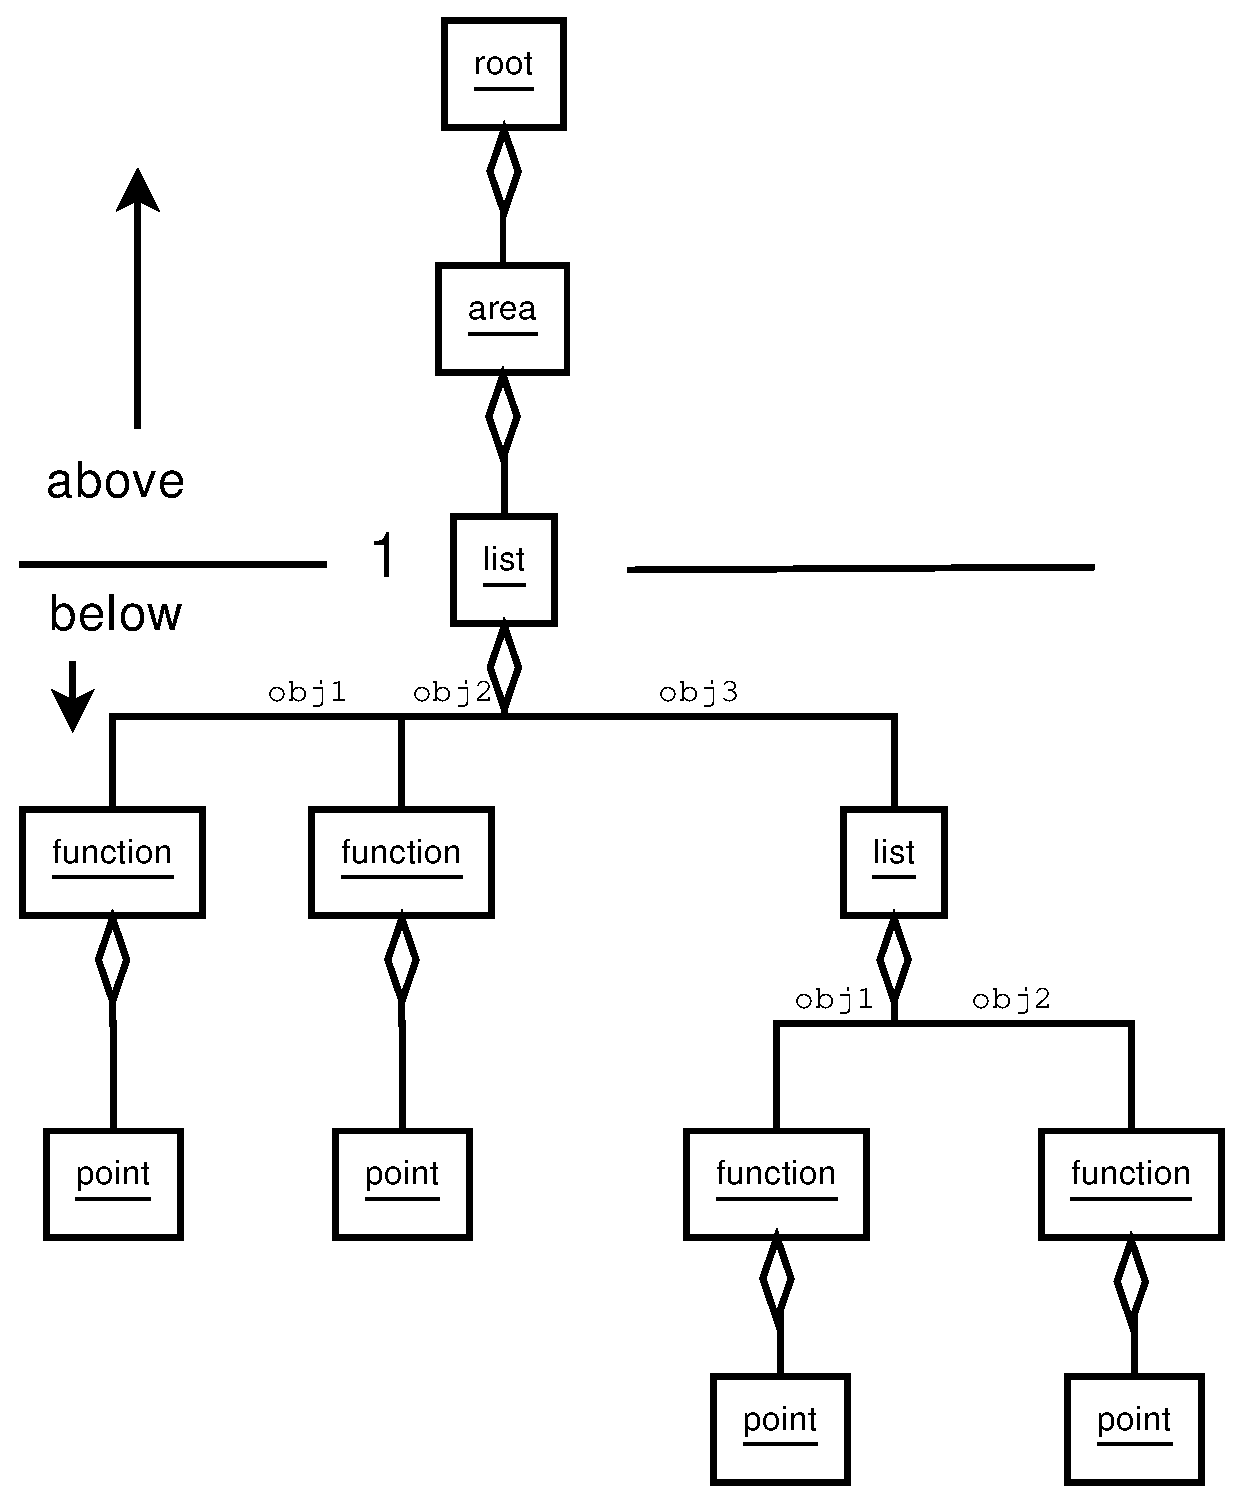
\includegraphics[scale=0.5]{above_below}
\end{center}
\caption{Example for ``below'' and ``above'' in a Fib object}
\label{figDirectionFibElements}
\end{figure}


\subsection{Order of the Fib elements}\index{order!Fib elements}
\label{secOrderFibElements}

On the definitions of ``below'' and ``above'' in a Fib object the order of Fib elements is established. To each Fib element in the complete Fib object an unique natural number is assigned. If in a Fib object $N$ elements exist, the numbers $1$ to $N$ will be assigned to the Fib elements in the Fib object. Fib elements below a Fib element are assigned to higher values.

If a list element subobject $Obj_U$ has a higher number $U$ as another subobject $Obj_K$ ($U>K$) of the list element, it also contains Fib elements with higher numbers as the Fib elements in $Obj_K$. The root-elements are treated the same way in the order as list elements, with the main-Fib-object as the first subobject after which the sub-root-objects follow in ther succession (in the root-element).

The same applies for any other branch element. The above defined syntax determines the order of the subobjects.

In figure \ref{figOrderFibElements} a sample object with the corresponding numbers (next to the elements) for the order of the Fib element is shown.

\begin{figure}[htbp]
\begin{center}
  \includegraphics[scale=0.5]{order_elements}
\end{center}
\caption{Example: Order of the Fib elements}
\label{figOrderFibElements}
\end{figure}


\subsection{Order of particular Fib elements}\index{Order!particular Fib elements}

Also Fib elements of a given typs are assigned to natural numbers of an order for there type. These orders are based on the order of the Fib elements. If in a correct Fib object $N$ Fib elements of a type exist, the numbers $1$ to $N$ are assigned to the Fib elements of this type. If to a Fib element $Elm_1$ in the order of the Fib elements a higher value is assigned (as to another Fib element $Elm_2$ of the same type), so it ($Elm_1$) is assigned to a higher value in the order of the Fib elements of the same type (than the other Fib element $Elm_2$).

In figure \ref{figOrderSpecialFibElements} an example object with the corresponding numbers (next to the elements) for the order of particular Fib element is shown.

\begin{figure}[htbp]
\begin{center}
  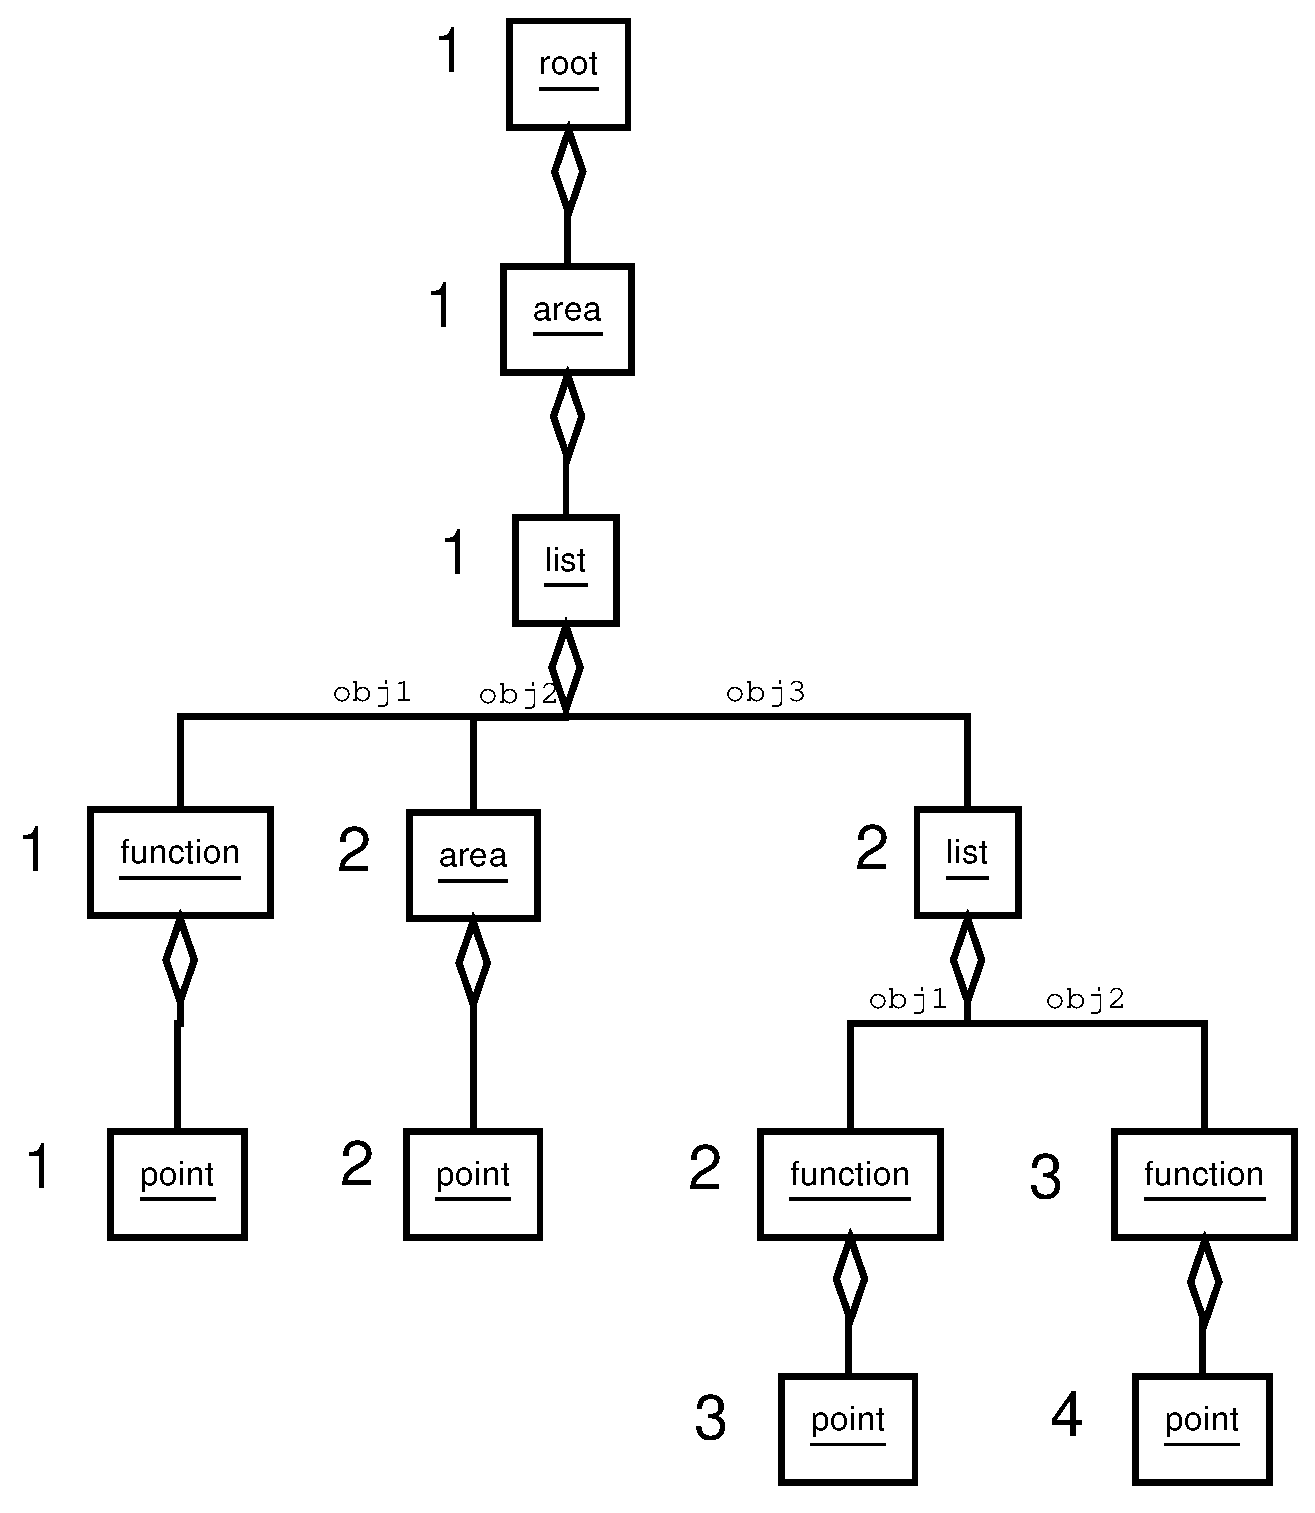
\includegraphics[scale=0.5]{order_special_elements}
\end{center}
\caption{Example: Order of particular Fib elements}
\label{figOrderSpecialFibElements}
\end{figure}


\subsection{Order of move points}\index{move points}\index{order!move points}

Another order applies to all Fib elements that can be moved. These are called move points.
The orders of the move points is based on the order of the Fib elements. If in a complete Fib object $N$ move points (movebel Fib elements) exist, the numbers $1$ to $N$ are assigned to these movebel Fib elements. If to a movebel Fib element $Elm_1$ in the order of the Fib elements a higher value is assigned (as to another movebel Fib element $Elm_2$), so it ($Elm_1$) is assigned to a higher value in the order of the movebel Fib elements (than the other Fib element $Elm_2$).

\bigskip\noindent
Fib elements, which can be moved and represent move points, are all limb elements (they are containing exactly one subobject):
\begin{itemize}
 \item property element (see section \ref{fibProperty} on page \pageref{fibProperty})
 \item comment element (see section \ref{fibComment} on page \pageref{fibComment})
 \item area element (see section \ref{fibArea} on page \pageref{fibArea})
 \item functions (see section \ref{fibFunction} on page \pageref{fibFunction})
 \item Fib elements, to retrive domain properties (see sectiont \ref{fibDomeinProperties} on page \pageref{fibDomeinProperties})
 \item set-element (see section \ref{secFibSetElement} on page \pageref{secFibSetElement})
 \item matrix element (see section \ref{secFibMatrixElement} on page \pageref{secFibMatrixElement})
\end{itemize}

\bigskip\noindent
Fib elements, which can't be moved and don't represent move points, are:
\begin{itemize}
 \item all leaf elements:
 \begin{itemize}
  \item points (see section \ref{fibPoint} on page \pageref{fibPoint})
  \item Fib elements to call external subobjects (see section \ref{fibSubobject} on page \pageref{fibSubobject})
 \end{itemize}
 \item all branch elements:
 \begin{itemize}
  \item root-element (see section \ref{fibRootElement} on page \pageref{fibRootElement})
  \item list element (see section \ref{fibList} on page \pageref{fibList})
  \item the Fib element, to call external objects (see section \ref{fibExtObject} on page \pageref{fibExtObject})
  \item conditions with the if-element (see section \ref{secFibIf} on page \pageref{secFibIf})
 \end{itemize}
\end{itemize}

In figure \ref{figOrderMovePoints} an example object with the corresponding numbers (next to the elements) for the order of move points is shown.

\begin{figure}[htbp]
\begin{center}
  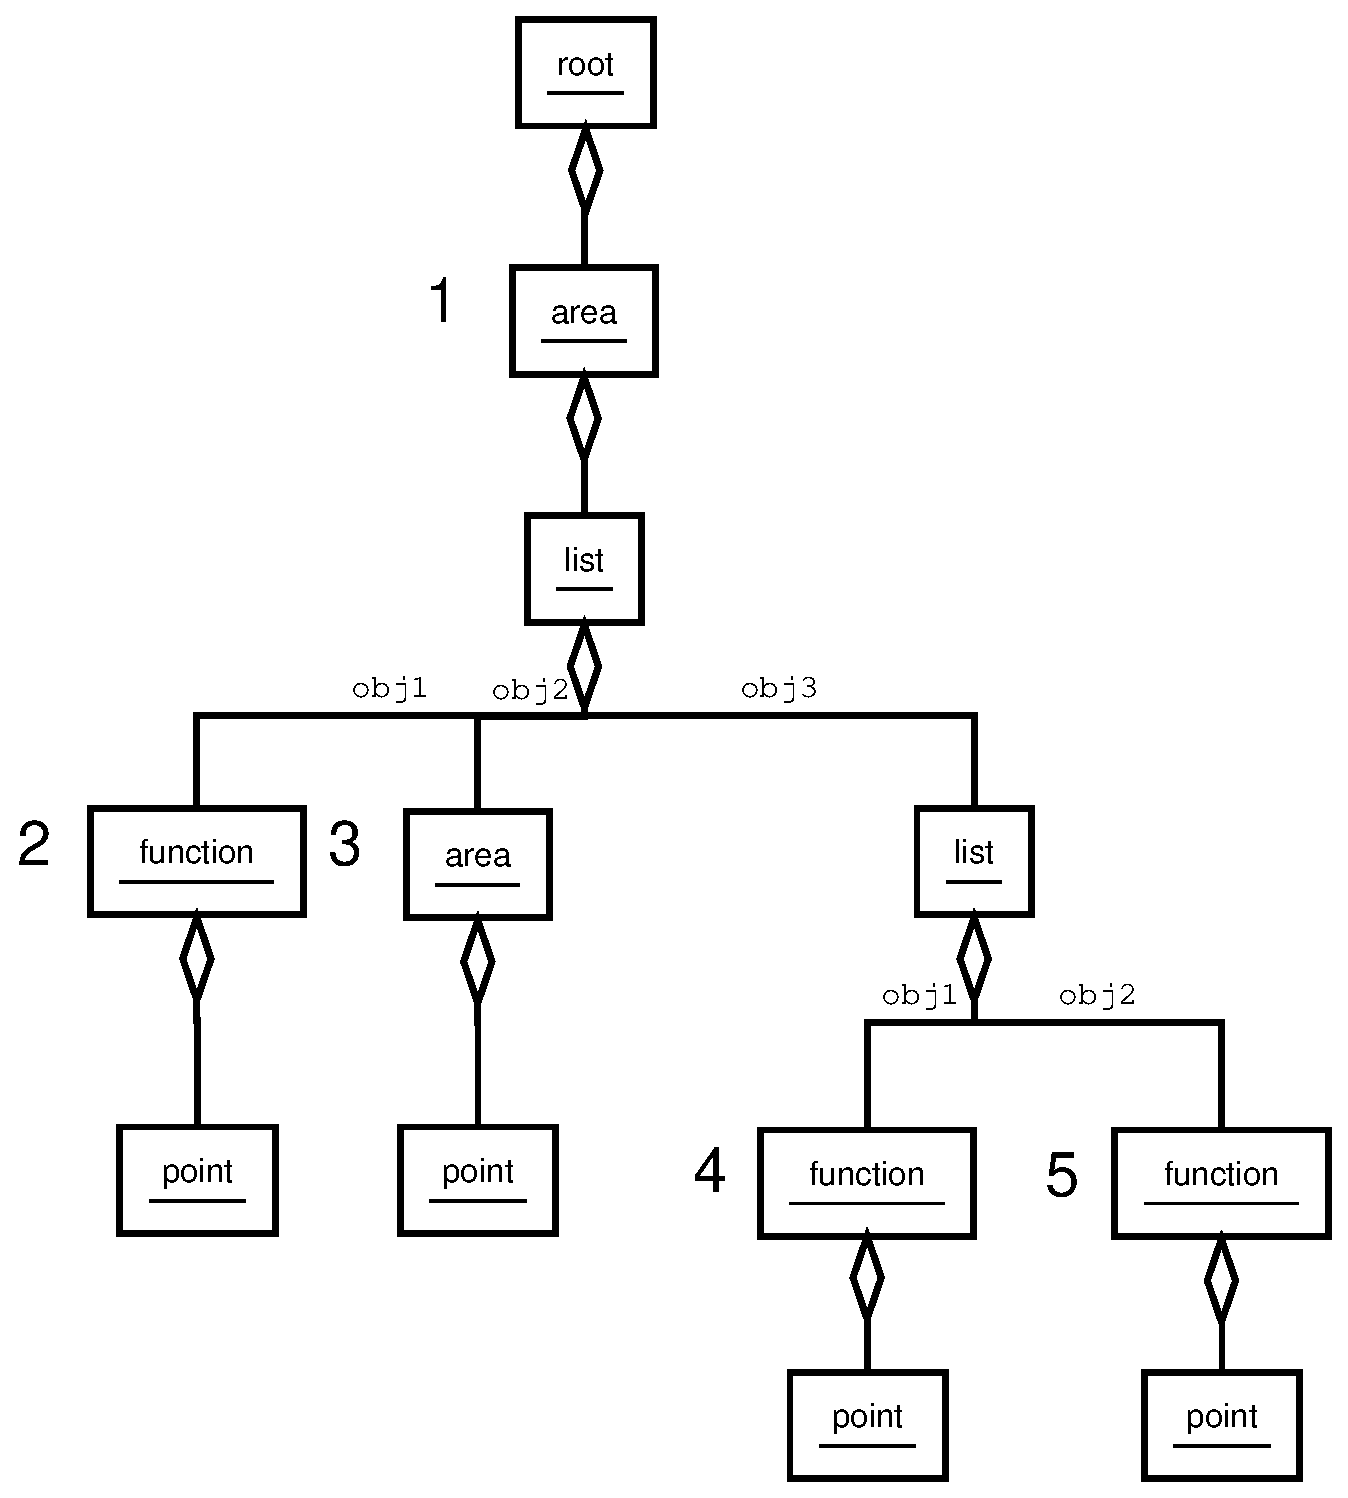
\includegraphics[scale=0.5]{order_move_points}
\end{center}
\caption{Example: Order of move points}
\label{figOrderMovePoints}
\end{figure}


\subsection{Definition: part object}\index{part object|(}

Any object that is a whole branch (e. g. a sub-list object, main-Fib-object or sub-root-object) of a branch element is part of a part object. Furthermore, to the part object belong all root-elements, in which it is contained or which it uses for external objects. Even Fib elements, which define variables that are used in the part object, belong to it.
The union of two part objects is again a part object.
The complete Fib object itself is also a part object.
A part object can always be evaluated to a multimedia object.

A \textbf{genuine part object}\index{part object!genuine} is a part object, that is not the (complete) Fib object itself.

A \textbf{simple part object}\index{part object!simple} is a genuine part object, that contains only one leaf with one point object.

A \textbf{coherent part object}\index{part object!coherent} is a genuine part object that contains the whole object of one branch (subobject), of just one branch element (e. g. list element or root-element) and the required elements above it. In particular, every simple object is a coherent subobject.

To create a coherent part object, one branch element (for example list element or root-element) from the complete Fib object can be deleted and replaced by one of the subobjects contained in it. The resulting subobject must of course be correct, to be a coherent part object. (For example, if the main-Fib-object of a root-element is deleted, the result isn't a coherent part object. Also if a sub-root-element is deleted, and the next above main-Fib-object is replaced by its main-Fib-object, the domains of the replace root-element should be adapted by the next root-element.)

With figure \ref{figOrderFibElementsPartobjects} this definition is illustrated with an example of a Fib object. In the following, some examples of different types of part objects in Figure \ref{figOrderFibElementsPartobjects} are being given, for the Fib elements their numbers (from the Fib element order respectively figure \ref{figOrderFibElementsPartobjects}) are given. Furthermore, it is establish that the point element with the number $10$ does not use the variable that is defined by the area element with the number $2$. All other variables are needed in the points, which are below the respective variable definitions.


\begin{figure}[htbp]
\begin{center}
  \includegraphics[scale=0.5]{order_elements}
\end{center}
\caption{Example object for part objects}
\label{figOrderFibElementsPartobjects}
\end{figure}


\bigskip\noindent
Part objects:
\begin{itemize}
 \item 1; 2; 4; 5
 \item 1; 2; 6; 7
 \item 1; 2; 3 (just subobjects $1$ and $2$); 4; 5; 6; 7
 \item 1; 9; 10
 \item 1; 2; 8; 9; 10; 11; 12
 \item 1; 2; 3 (just subobjects $1$ and $3$); 4; 5; 8; 9; 10; 11; 12
 \item 1; 2; 3 (just subobjects $1$ and $3$); 4; 5; 11; 12
 \item (all Fib elements) 1; 2; 3; 4; 5; 6; 7; 8; 9; 10; 11; 12
\end{itemize}

Genuine part objects:
\begin{itemize}
 \item 1; 2; 4; 5
 \item 1; 2; 6; 7
 \item 1; 2; 3 (just subobjects $1$ and $2$); 4; 5; 6; 7
 \item 1; 9; 10
 \item 1; 2; 8; 9; 10; 11; 12
 \item 1; 2; 3 (just subobjects $1$ and $3$); 4; 5; 8; 9; 10; 11; 12
 \item 1; 2; 3 (just subobjects $1$ and $3$); 4; 5; 11; 12
\end{itemize}

Simple part objects:
\begin{itemize}
 \item 1; 2; 4; 5
 \item 1; 2; 6; 7
 \item 1; 9; 10
 \item 1; 2; 11; 12
\end{itemize}

Coherent part objects:
\begin{itemize}
 \item 1; 2; 4; 5
 \item 1; 2; 6; 7
 \item 1; 9; 10
 \item 1; 2; 11; 12
 \item 1; 2; 8; 9; 10; 11; 12
\end{itemize}


\subsection{Order of the coherent part objects}
\label{secOrderPartobjects}

There is an order on the coherent part objects as well. This will hereinafter also called order of part objects, as there are no own orders for the other types of part objects.

The orders of the (coherent) part objects is based on the order of the Fib elements. If in a complete Fib object $N$ (coherent) part objects exist, the numbers $1$ to $N$ are assigned to these part objects.
The greater the number of a coherent part object, the greater is the smallest number in order of the Fib elements, of the Fib elements in it.
Or: If to the top most Fib element of the subobject, which defines the coherent part object, a higher value assigned, than the defined part object is also associated with a higher value.

In figure \ref{figOrderPartobjekts} an example object with the corresponding numbers (next to the defining subobjects of the part objects) for the order of (coherent) part objects is shown.

\begin{figure}[htbp]
\begin{center}
  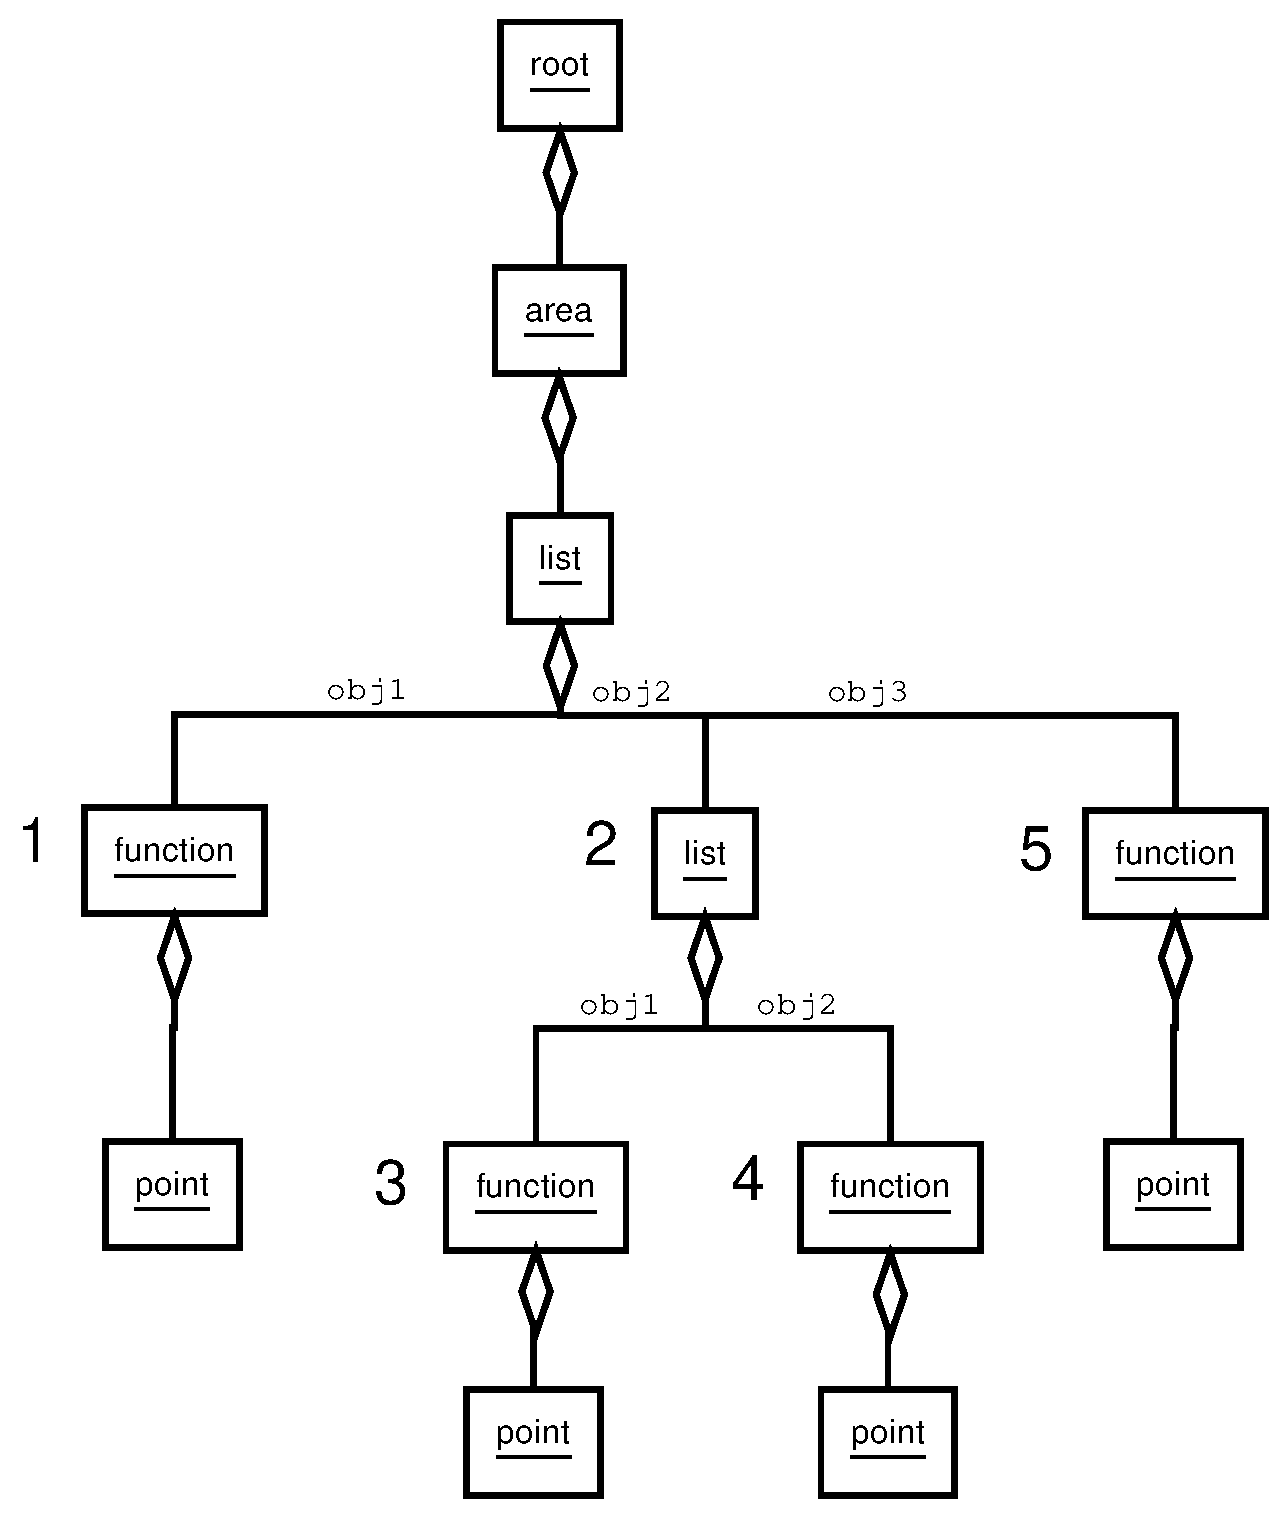
\includegraphics[scale=0.5]{order_partobjects}
\end{center}
\caption{Example: Order of (coherent) part objects}
\label{figOrderPartobjekts}
\end{figure}


\index{part object|)}


\subsection{Definition of Fib multimedia object}\index{Fib multimedia object}

If the expression Fib multimedia object is used, the Fib object with focus on the multimedia object it represents is meant.


\subsection{Definition of correct Fib multimedia object}\index{Fib multimedia object!correct}

A correct Fib multimedia object is a Fib object, that fully reflects the original multimedia object, which it should represent. So, if the multimedia object that the Fib object represents, and the original multimedia object are compared, no difference between them can be found.



%TODO: in welche Sprache kontextfrei oder regulär?




